\documentclass[12pt,a4paper]{article}
\usepackage[utf8]{inputenc}
\usepackage{amsmath}
\usepackage{amsfonts}
\usepackage{amssymb}
\usepackage{graphicx}
\usepackage{dirtree}
\usepackage[spanish]{babel}
\usepackage{color}
%%%%%%%%%%%%%%%%%%%%%%%%%%%%%% User specified LaTeX commands.
\makeatletter\makeatother
\usepackage{listings}
\usepackage{subfig}
\usepackage{float}

% Paketea konfiguratu behar dugu C lengoaiarekin erabiltzeko:
\definecolor{darkgreen}{rgb}{0,0.5,0}
\definecolor{lightgray}{rgb}{0.95,0.95,0.95}
\definecolor{gray}{rgb}{0.65,0.65,0.65}
\lstset{language=C,
		basicstyle=\scriptsize\ttfamily\tiny,
		keywordstyle=\color{darkgreen}\bfseries,
		identifierstyle=\color{blue},
		commentstyle=\color{gray}, 
		stringstyle=\ttfamily,
		showstringspaces=false,
		tabsize=2,
		backgroundcolor=\color{lightgray}}


\begin{document}

\title{\begin{center}
\resizebox*{0.50\textwidth}{0.15 \textheight}{

\includegraphics{images/ehu-pdf}
} 
\end{center}
\vspace{1cm}
Documentación técnica}

\author{Leroy Deniz}

\maketitle
\begin{abstract}
La aplicación pretende ser un motor gráfico.  En ella se pueden insertar objetos en 3D,  aplicarles transformaciones, elegir y manipular cámaras, así como modificar las luces y los materiales. 

Se explica en este documento las estructuras básicas necesarias para el correcto funcionamiento de la aplicación y las funciones destacadas que permiten su uso.

Además, se adjuntan capturas de pantalla para permitir una mayor compresión de la aplicación y su funcionamiento, y un apartado específico de manejo de usuario que facilite su uso.

\end{abstract}

\vspace{2cm}

\begin{center}
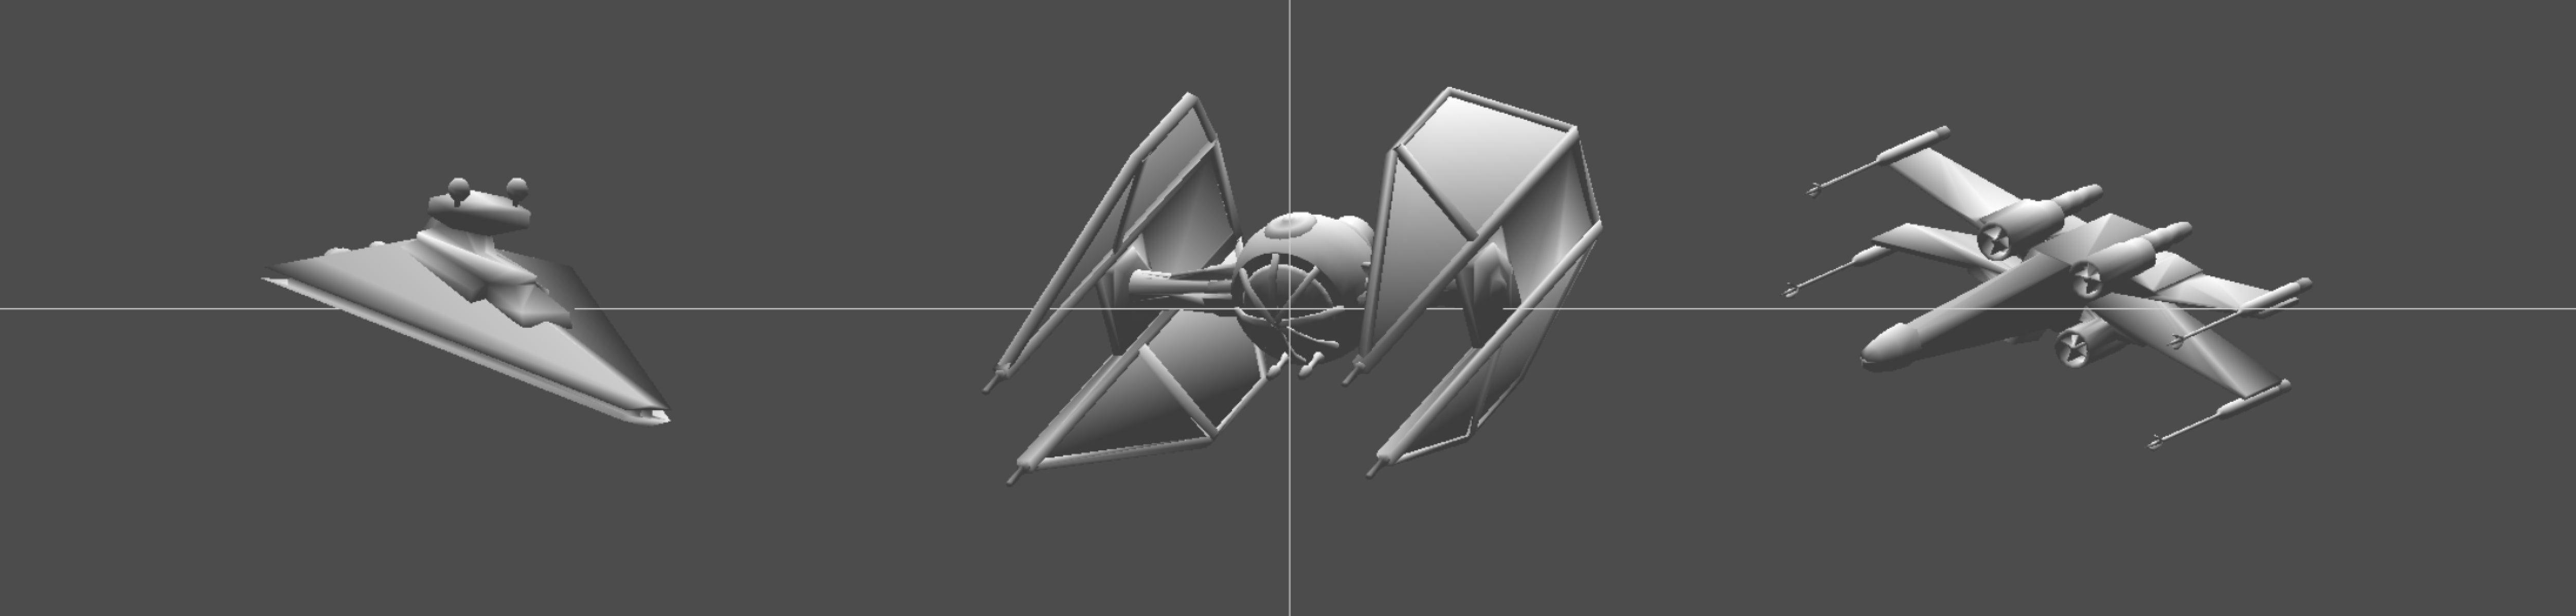
\includegraphics[width=14cm]{images/portada}
\end{center}


\newpage
\tableofcontents





\newpage

\section{Requerimientos funcionales}

Para poder compilar y ejecutar esta aplicación, hacen falta una serie de librerías que se deben instalar, para este caso utilizaremos como sistema operativo Debian 10, distribución gratis de Linux.

Instalación de las librerías de OpenGL.

\begin{verse}
\begin{verbatim}
$ aptitude install freeglut3 freeglut3-dev
\end{verbatim}
\end{verse}

Instalación de la suite $ImageMagik$ para edición de imágenes en modo consola.

\begin{verse}
\begin{verbatim}
$ aptitude install imagemagik
\end{verbatim}
\end{verse}

Instalación del compilador $gcc$ para linux

\begin{verse}
\begin{verbatim}
$ aptitude install gcc
\end{verbatim}
\end{verse}

\vspace{1cm}
Una vez instaladas todas las dependencias, la instrucción para compilar la aplicación, estando en el directorio donde se encuentran los archivos, es:

\begin{verse}
\begin{verbatim}
$ gcc *.c -lGL -lGLU -lglut -lm -o app
\end{verbatim}
\end{verse}









\newpage
\section{Estructura de ficheros}

\subsection{Estructura}

La aplicación se constituye en base a los siguientes ficheros.  Además se agrega un directorio con objetos grandes en 3D para poder ver el funcionamiento de la aplicación.

\vspace{0.5cm}
\dirtree{%
 .1 /.
 .2 a.out.
 .2 camara.c.
 .2 camara.h .
 .2 definitions.h.
 .2 display.c.
 .2 display.h.
 .2 docs.
 .3 manual.pdf.
 .2 io.c.
 .2 io.h.
 .2 load\_obj.h.
 .2 load\_obj\_joseba.c.
 .2 main.c.
 .2 obj.
 .3 A380.obj.
 .3 altair.obj.
 .3 deathstr.obj.
 .3 destroyr.obj.
 .3 dinodragon.obj.
 .3 intercep.obj.
 .3 r\_falke.obj.
 .3 \dots .
  }

\vspace{0.5cm}

\subsection{Descripción de ficheros}

Se adjunta una breve explicación de la responsabilidad de cada fichero.

\begin{itemize}
  \item \texttt{a.out}: ejecutable de la aplicación.
  \item \texttt{camara.c}: define las funciones para manejo de cámaras.
  \item \texttt{camara.h}: contiene los cabezales de las funciones implementadas en \texttt{camara.c}.
  \item \texttt{definitions.h}: contiene las estructuras necesarias para la implementación de los objetos a utilizar
  \item \texttt{display.c}: es donde se implementan las vistas, decide qué se muestra y cómo lo hace. Es quien dibuja.
  \item \texttt{display.h}: tiene las definiciones de las funciones a implementar en \texttt{display.c}.
  \item \texttt{io.c}: responsable de controlar las entradas por teclado de las órdenes del usuario, de seleccionar la acción requerida, implementa las funciones y procedimientos y delega la responsabilidad de mostrar en \texttt{display.h}.
  \item \texttt{io.h}: define los cabezales de las funciones implementadas en \texttt{io.c}.
  \item \texttt{load\_obj.h}: define los cabezales de las funciones implementadas en \texttt{load\_obj\_joseba.c}.
  \item \texttt{load\_obj\_joseba.c}: es donde se definen las funciones que permiten cargar el objeto de un archivo a memoria.
  \item \texttt{io.h}: define los cabezales de las funciones implementadas en \texttt{io.c}.
  \item \texttt{main.c}: define el programa principal e inicializa el estado de situación sobre el que se va a trabajar. El título de la ventana,  el tamaño, etc.
\end{itemize}













\newpage

\section{Interacción usuario-aplicación}
Para sintetizar las teclas de control que permite el sistema, adjuntamos una captura de pantalla de la función de ayuda.


\subsection{Función de ayuda}

Se adjunta su código fuente implementado en \texttt{io.c}, que responde a la tecla \texttt{?}.
\vspace{0.5cm}

\begin{lstlisting}
void print_help() {
	printf("*** Practica GC - Leroy Deniz ***\n\n");

	printf("*** FUNCIONES PRINCIPALES ***\n");
	printf("<?>\t\t Mostrar la ayuda \n");
	printf("<ESC>\t\t Salir del programa \n");
	printf("<F>\t\t Cargar un objeto\n");
	printf("<TAB>\t\t Cambiar objeto seleccionado\n");
	printf("<DEL>\t\t Eliminar objeto\n\n");
	printf("<CTRL + ->\t Alejar\n");
	printf("<CTRL + +>\t Acercar\n");
	printf("<CTRL + Z z>\t Deshacer\n");
	printf("<CTRL + X x>\t Rehacer\n\n");
	printf("<UP>\t\t Trasladar+Y | Escalar+Y | Rotar+X \n");
	printf("<DOWN>\t\t Trasladar-Y | Escalar-Y | Rotar-X \n");
	printf("<RIGHT>\t\t Trasladar+X | Escalar+X | Rotar+Y \n");
	printf("<LEFT>\t\t Trasladar-X | Escalar-X | Rotar-Y \n");
	printf("<AVPAG>\t\t Trasladar+Z | Escalar+Z | Rotar+Z \n");
	printf("<REPAG>\t\t Trasladar-Z | Escalar-Z | Rotar-Z \n");
	printf("\n\n");

	printf("*** SELECCION DE MODOS ***\n");
	printf("<CTRL + O o>\t\t Modo objeto \n");
	printf("<CTRL + K k>\t\t Modo camara \n");
	printf("<CTRL + A a>\t\t Modo luz \n");
	printf("\n\n");

	printf("*** FUNCIONES TRANSFORMACION ***\n");
	printf("<CTRL + M m>\t\t Modo traslacion \n");
	printf("<CTRL + B b>\t\t Modo rotacion \n");
	printf("<CTRL + T t>\t\t Modo escalado \n");
	printf("<CTRL + G g>\t\t Sistema de referencia global \n");
	printf("<CTRL + L l>\t\t Sistema de referencia local \n");
	printf("\n\n");

	printf("*** FUNCIONES DE CAMARA ***\n");
	printf("<c>\t\t Cambia la camara \n");
	printf("<C>\t\t Visualizacion desde el objeto \n");
	printf("<n>\t\t Anadir nueva camara \n");
	printf("<G g>\t\t Camara en modo analisis \n");
	printf("<L l>\t\t Camara en modo vuelo\n");
	printf("<T t>\t\t Cambio de volumen de vision \n");
	printf("<B b>\t\t Rotacion de la camara \n");
	printf("<M m>\t\t Traslacion de la camara \n");
	printf("<P p>\t\t Cambio de proyeccion: perspectiva / paralela \n");
	printf("\n\n");

	printf("*** FUNCIONES ILUMINACION ***\n");
	printf("<F1>\t\t Activar / desactivar SOL \n");
	printf("<F2>\t\t Activar / desactivar BOMBILLA \n");
	printf("<F3>\t\t Activar / desactivar FOCO DEL OBJETO \n");
	printf("<1 - 8>\t\t Seleccionar fuente de luz correspondiente \n");
	printf("<F9>\t\t Activar / desactivar iluminacion \n");
	printf("<F12>\t\t Cambiar tipo de iluminacion \n");
	printf("<+>\t\t Incrementar angulo de apertura de foco\n");
	printf("<->\t\t Decrementar angulo de apertura de foco\n");
	printf("\n\n");
}

\end{lstlisting}

\newpage
Vista de la función de ayuda en la ejecución del programa.

\begin{center}
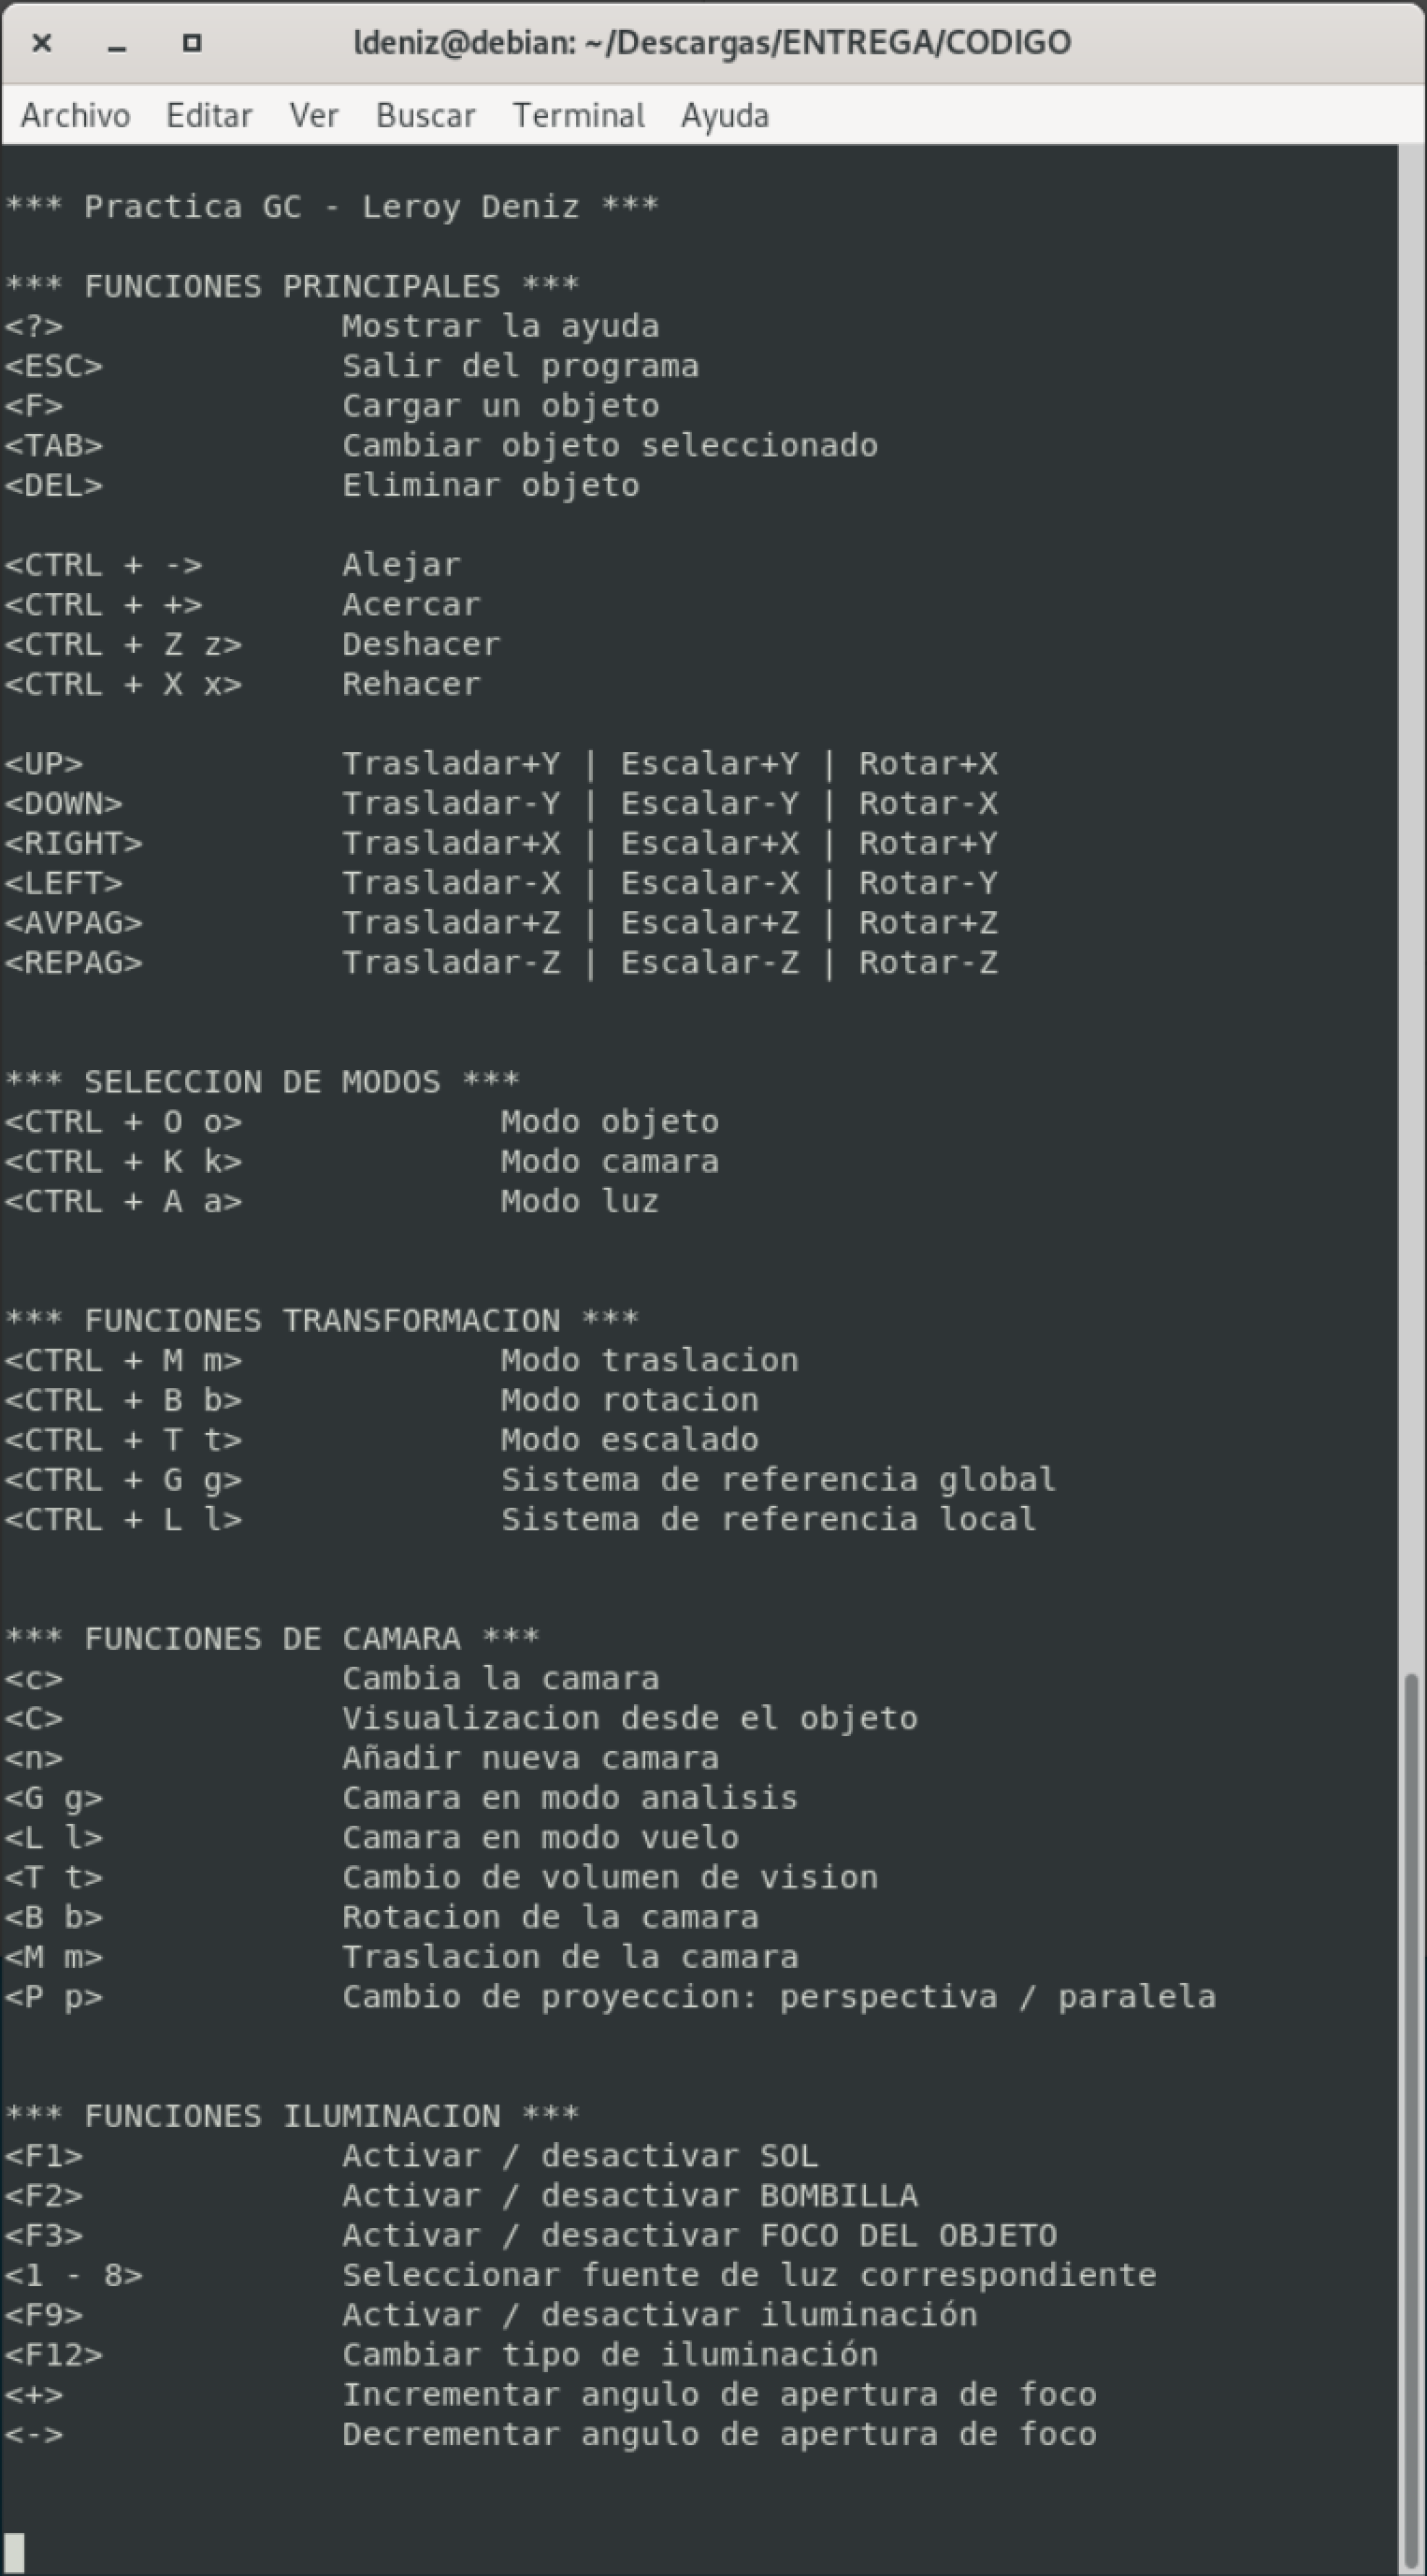
\includegraphics[width=9cm]{images/ayuda}
\end{center}


\newpage
\subsection{Consideraciones importantes en el uso}

\subsubsection{Unicidad de elemento y acción}
Los modos global y local sin excluyentes entre sí,  no se puede trabajar en ambos modos al mismo tiempo; así como las funciones de traslación, rotación y escalado también excluyentes entre sí, habilitar uno implica necesariamente deshabilitar los demás. De la misma forma ocurre con los objetos que se están seleccionando, se selecciona un único objeto entre Objeto 3D, cámara o Luz.

\subsubsection{Opciones por default}

Al seleccionar un objeto se activan por default su modo local de trabajo y la rotación. Cuando se selecciona una cámara, se activa en modo local y con traslación Cuando se selecciona Luz, se selecciona el modo local y la traslación del objeto de iluminación que corresponda. El material por defecto es Jade.


\subsubsection{Diferencia entre cámaras}
Modo vuelo permite la libertad de movimiento del objeto cámara por cualquier parte del mundo, sin embargo, el modo análisis se mueve únicamente sobre una esfera que rodea el objeto, por lo que siempre estará mirando al centro del objeto, moviéndose hacia los lados, alejándose o acercándose,







\newpage
\section{Estructuras de objetos}

Las estructuras están definidas en el archivo \texttt{definitions.h},  donde tenemos lo siguiente:

\subsection{Estructuras básicas}

Aquellas estructuras que venían definidas en el proyecto desde la base, sobre la cual se construye el resto de la aplicación.

% entorno lstlisting para escribir código
\begin{lstlisting}
/****************************
 * Structure to store the   *
 * coordinates of 3D points *
 ****************************/
typedef struct {
    GLdouble x, y, z;
} point3;

/*****************************
 * Structure to store the    *
 * coordinates of 3D vectors *
 *****************************/
typedef struct {
    GLdouble x, y, z;
} vector3;

/****************************
 * Structure to store the   *
 * colors in RGB mode       *
 ****************************/
typedef struct {
    GLfloat r, g, b;
} color3;

/****************************
 * Structure to store       *
 * objects' vertices        *
 ****************************/
typedef struct {
    vector3 normal;
    point3 coord;        /* coordinates,x, y, z */
    GLint num_faces;     /* number of faces that share this vertex */
} vertex;

/****************************
 * Structure to store       *
 * objects' faces or        *
 * polygons                 *
 ****************************/
typedef struct {
    vector3 normal;
    GLint num_vertices;     /* number of vertices in the face */
    GLint *vertex_table;    /* table with the index of each vertex */
} face;

\end{lstlisting}


\newpage
\subsection{Estructuras complementarias}

Son aquellas que definen los objetos principales de la aplicación: objetos 3D,  cámaras,  materiales y luces.  Para poder definir una lista de cambios sobre un objeto,  definimos una estructura \texttt{elem\_Matriz} que tendrá una matriz y un puntero a otra estructura igual.  De esta forma,  estamos consiguiendo una lista de matrices ordenadas,  que inician en la primera transformación sobre un objeto y finaliza en la situación actual. Esto permite poder implementar las funciones de hacer y deshacer.

% entorno lstlisting para escribir código
\begin{lstlisting}
/****************************
 * Estructura de matriz     *
 ****************************/
typedef struct elem_Matriz{
    GLdouble M[16];                /*matriz de la tranformacion*/
    struct elem_Matriz *siguiente; /*Puntero al siguiente nodo*/
} elem_Matriz;

/****************************
 * Estructura de objetos    *
 ****************************/
struct object3d{
    GLint num_vertices;            /* number of vertices in the object*/
    vertex *vertex_table;          /* tabla de vertices */
    GLint num_faces;               /* numero de caras del objeto */
    face *face_table;              /* tabla de caras */
    point3 min;                    /* coordinates' lower bounds */
    point3 max;                    /* coordinates' bigger bounds */
    material mt;			    /* definicion del material sobre el objeto */
    elem_Matriz *pMptr;            /* puntero a la matriz de transformaciones*/
    elem_Matriz *containerNodePtr; /* puntero al primer nodo containerNode*/
    struct object3d *siguiente;    /* puntero al siguiente objeto */
};

/****************************
 * Estructura de materiales *
 ****************************/
typedef struct material{
	GLfloat ambient[4];
	GLfloat diffuse[4];
	GLfloat specular[4];
	GLfloat shininess;
}material;

/****************************
 * Estructura de camaras    *
 ****************************/
typedef struct camara{
    point3 e;
    point3 at;
    vector3 up;
    GLdouble matrizCamara[16];
} camara;

/****************************
 * Estructura de luces      *
 ****************************/
typedef struct luz{
    int tipo;
    int estado;
    GLfloat pos[4];
    GLfloat dir[3];
    GLfloat ambient[4];
    GLfloat diffuse[4];
    GLfloat specular[4];
    GLfloat ampFoco;
} luz;

typedef struct object3d object3d;

\end{lstlisting}










\newpage
\section{Transformaciones geométricas}

\subsection{Matriz de representación del objeto}

Cada objeto 3D tiene una matriz de representación que permite implementar las funciones de Undo y Redo. Para ello, es necesario que cada objeto almacene las matrices asociadas a todas las transformaciones que se le aplicaron, para poder ser deshechas o rehechas. 

\texttt{M} es un vector de 16 posiciones donde se almacena la matriz resultado de la aplicación de las transformaciones.  Como se utilizan objetos de tres dimensiones, se utilizan matrices de 4x4.

Además, \texttt{*siguiente} es un puntero al siguiente nodo de la lista, que resultará en la dirección de la siguiente matriz de transformación sobre el objeto seleccionado.

\begin{lstlisting}
/****************************
 * Estructura de matriz     *
 ****************************/

typedef struct elem_Matriz{
    GLdouble M[16];                /*matriz de la tranformacion*/
    struct elem_Matriz *siguiente; /*Puntero al siguiente nodo*/
} elem_Matriz;

\end{lstlisting}

Es necesario contar un un puntero que referencie a la última transformación del objeto, que tendrá la matriz de transformaciones final y será la que OpenGL muestre por pantalla. Es esencial para la implementación de Redo y Undo.

Para la inicialización, se reserva espacio en memoria con \texttt{malloc()} y luego cargar en la lista un nodo con la matriz identidad. Esto se hace en el momento de la carga inicial del objeto, ya que con posteriores transformaciones, esta matriz irá cambiando. Cada vez que se pulsa la tecla F, el sistema permite ingresar la ruta a un nuevo objeto (fichero de extensión .obj). La función que maneja esta funcionalidad está en \texttt{io.c} y se llama \texttt{keyboard()}.

Es necesario ahora, para dibujar los objetos, sustituir la matriz identidad por la matriz de transformacion. Esa será la matriz que apunte el puntero \texttt{pMptr} del objeto seleccionado.

\vspace{0.5cm}
\begin{lstlisting}
//muestra el objeto con la ultima transformacion realizada (acumulada)
glLoadMatrixd(_selected_object->pMptr->M);

\end{lstlisting}

\newpage

Una vez cargada la imagen al entorno, se puede visualizar en la ventana de la siguiente manera:

\begin{center}
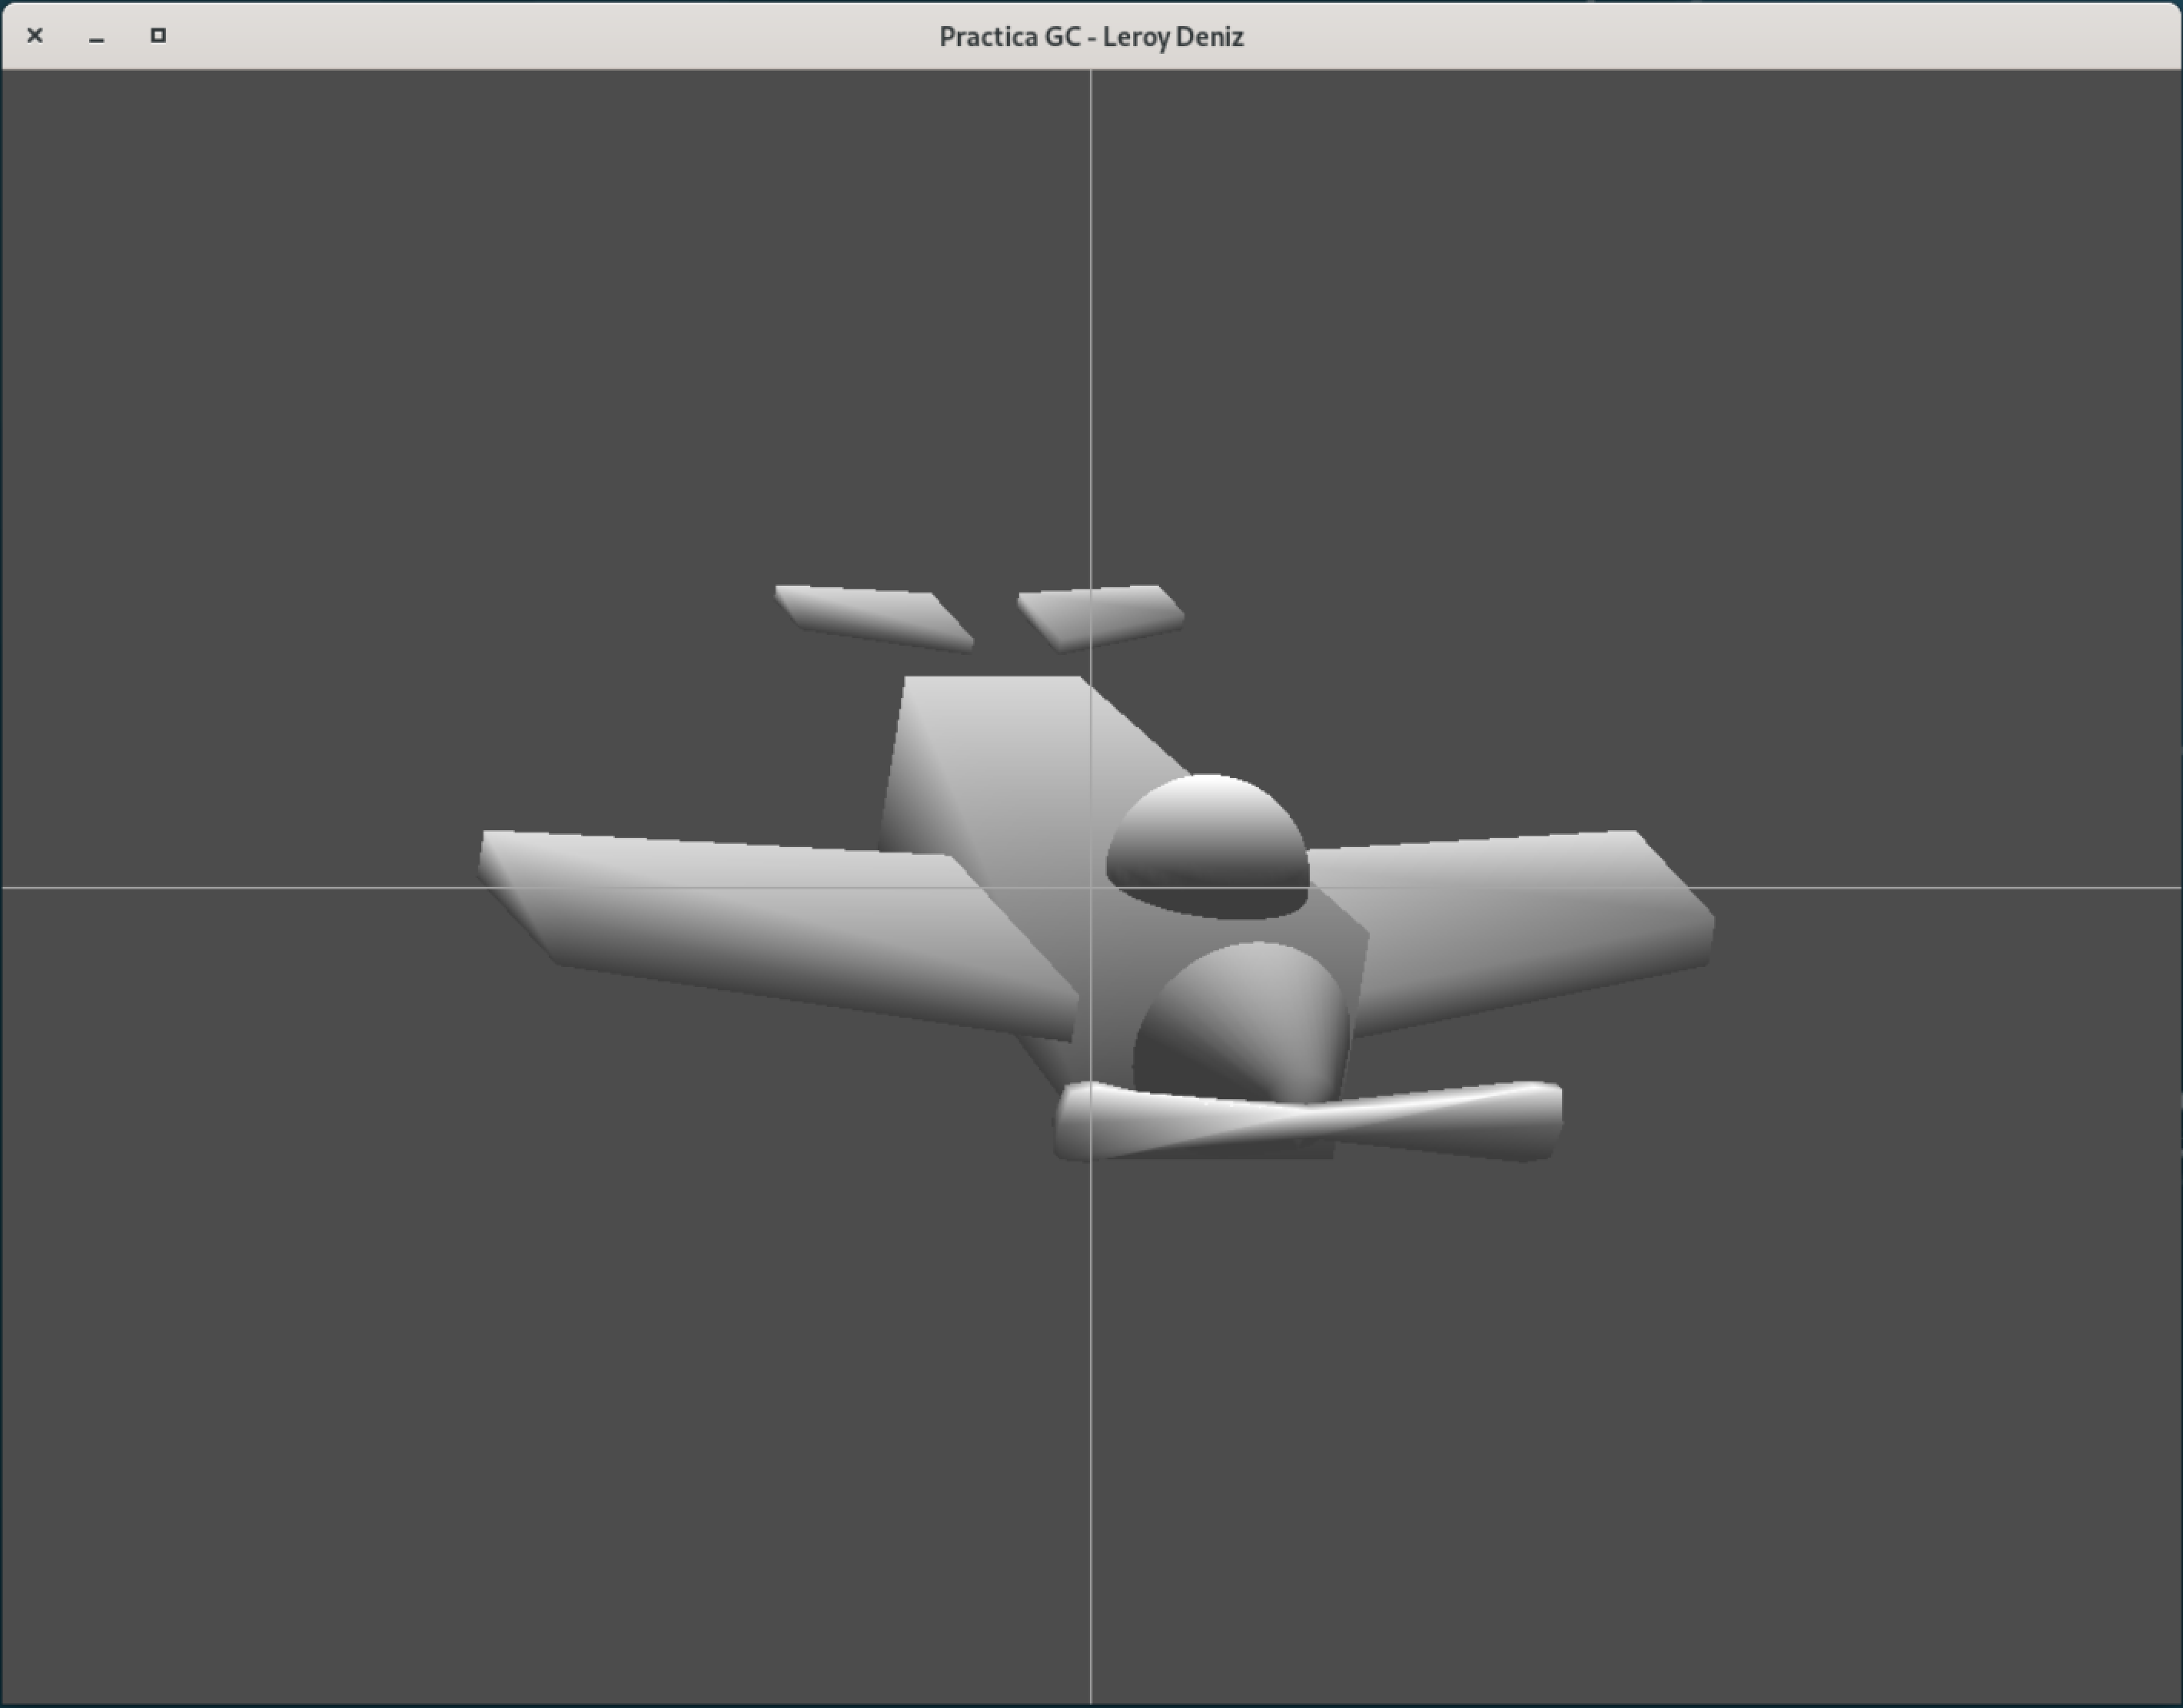
\includegraphics[width=10cm]{images/transformaciones}
\end{center}

\subsection{Constantes y valores}

Para controlar los modos y opciones de forma global, se establecen constantes y se predefinen sus valores como se muestra a continuación.

\vspace{0.5cm}
\begin{lstlisting}
#define ROTACION 0
#define ESCALADO 1
#define TRASLACION 2
#define VOLUMEN 3

#define GLOBAL 0
#define LOCAL 1

#define OBJETO 0
#define CAMARA 1
#define LUZ 2

\end{lstlisting}


\subsection{Sistema de referencia}

La definición del sistema de referencia se hace a través de las teclas G y L para global y local respectivamente. Esto permite al usuario poder realizar transformaciones en ambos sistemas, no limitándose a ninguno de ellos en particular.

\begin{itemize}
  \item \texttt{G}: cambiar al sistema de referencia global
  \item \texttt{L}: cambiar al sistema de referencia local
\end{itemize}

\subsection{Tipo de transformación}

La aplicación tiene implementada tres funcionalidades principales para la transformación de los objetos. Por un lado, la traslación del objeto, activándose con la tecla M, la rotación del mismo con la tecla B y el escalado con la tecla M. Las tres funcionalidades además, se aplican sobre ambos sistemas de referencia de forma disjunta.

\begin{itemize}
  \item \texttt{T}: Escalado
  \item \texttt{B}: Rotación
  \item \texttt{M}: Traslación
\end{itemize}

\subsection{Tipo de objeto}

Se puede elegir entre tres tipos de objetos para transformar; por un lado, transformaciones sobre un objeto 3D, cámara o luz.

\begin{itemize}
  \item \texttt{O}: Aplicar transformación sobre objeto actual
  \item \texttt{K}: Aplicar transformación sobre Cámara actual
  \item \texttt{A}: Aplicar transformación sobre Luz seleccionada
\end{itemize}


\subsection{Funciones de transformación}

\subsubsection{Funciones de rotación local}

La rotación local implica la utilización de coordenadas homogéneas para poder ejecutarla.

\begin{lstlisting}
/*********************************/
/*** FUNCION DE ROTACION LOCAL ***/
/*********************************/

void ejecutaRotacion(int key, int x, int y) {
    GLdouble rota_respecto_x_plus[16] = {1, 0, 0, 0, 0, cos(0.05), sin(0.05), 0, 0, -sin(0.05), 
    			cos(0.05), 0, 0, 0, 0, 1};
    GLdouble rota_respecto_x_minus[16] = {1, 0, 0, 0, 0, cos(-0.05), sin(-0.05), 0, 0, -sin(-0.05), 
    			cos(-0.05), 0, 0, 0, 0, 1};

    GLdouble rota_respecto_y_plus[16] = {cos(0.05), 0, -sin(0.05), 0, 0, 1, 0, 0, sin(0.05), 0, 
    			cos(0.05), 0, 0, 0, 0, 1};
    GLdouble rota_respecto_y_minus[16] = {cos(-0.05), 0, -sin(-0.05), 0, 0, 1, 0, 0, sin(-0.05), 0, 
    			cos(-0.05), 0, 0, 0, 0, 1};

    GLdouble rota_respecto_z_plus[16] = {cos(0.05), sin(0.05), 0, 0, -sin(0.05), cos(0.05), 0, 0, 
    			0, 0, 1, 0, 0, 0, 0, 1};
    GLdouble rota_respecto_z_minus[16] = {cos(-0.05), sin(-0.05), 0, 0, -sin(-0.05), cos(-0.05), 0, 0, 
    			0, 0, 1, 0, 0, 0, 0, 1};

    if (key == GLUT_KEY_UP) {
        multiplicaMatriz(rota_respecto_x_plus);
    } else if (key == GLUT_KEY_LEFT) {
        multiplicaMatriz(rota_respecto_y_minus);
    } else if (key == GLUT_KEY_DOWN) {
        multiplicaMatriz(rota_respecto_x_minus);
    } else if (key == GLUT_KEY_RIGHT) {
        multiplicaMatriz(rota_respecto_y_plus);
    } else if (key == GLUT_KEY_PAGE_UP) {
        multiplicaMatriz(rota_respecto_z_minus);
    } else if (key == GLUT_KEY_PAGE_DOWN) {
        multiplicaMatriz(rota_respecto_z_plus);
    }
}


\end{lstlisting}

\subsubsection{Funciones de escalado local}

Para ejecutar el escalado,  se multiplica cada vector del objeto por un escalar, manteniendo así las proporciones en el eje sobre el cual se escala.

\begin{lstlisting}

/*********************************/
/*** FUNCION DE ESCALADO LOCAL ***/
/*********************************/

void ejecutaEscalado(int key, int x, int y) {
    GLdouble escala_x_Plus[16] = {1.05, 0, 0, 0, 0, 1, 0, 0, 0, 0, 1, 0, 0, 0, 0, 1};
    GLdouble escala_x_Minus[16] = {0.95, 0, 0, 0, 0, 1, 0, 0, 0, 0, 1, 0, 0, 0, 0, 1};

    GLdouble escala_y_Plus[16] = {1, 0, 0, 0, 0, 1.05, 0, 0, 0, 0, 1, 0, 0, 0, 0, 1};
    GLdouble escala_y_Minus[16] = {1, 0, 0, 0, 0, 0.95, 0, 0, 0, 0, 1, 0, 0, 0, 0, 1};

    GLdouble escala_z_Plus[16] = {1, 0, 0, 0, 0, 1, 0, 0, 0, 0, 1.05, 0, 0, 0, 0, 1};
    GLdouble escala_z_Minus[16] = {1, 0, 0, 0, 0, 1, 0, 0, 0, 0, 0.95, 0, 0, 0, 0, 1};

    if (key == GLUT_KEY_UP) {
        multiplicaMatriz(escala_y_Plus);
    } else if (key == GLUT_KEY_LEFT) {
        multiplicaMatriz(escala_x_Minus);
    } else if (key == GLUT_KEY_DOWN) {
        multiplicaMatriz(escala_y_Minus);
    } else if (key == GLUT_KEY_RIGHT) {
        multiplicaMatriz(escala_x_Plus);
    } else if (key == GLUT_KEY_PAGE_UP) {
        multiplicaMatriz(escala_z_Minus);
    } else if (key == GLUT_KEY_PAGE_DOWN) {
        multiplicaMatriz(escala_z_Plus);
    }
}


\end{lstlisting}

\subsubsection{Funciones de traslación local}

Para efectuar la traslación en el Sistema de Referencia Local, se debe sumar el vector que corresponde a la traslación, a cada punto del objeto.

\begin{lstlisting}

/***********************************/
/*** FUNCION DE TRASLACION LOCAL ***/
/***********************************/

void ejecutaTraslacion(int key, int x, int y) {
    GLdouble tras_x_Plus[16] = {1, 0, 0, 0, 0, 1, 0, 0, 0, 0, 1, 0, 0.2, 0, 0, 1};
    GLdouble tras_x_Minus[16] = {1, 0, 0, 0, 0, 1, 0, 0, 0, 0, 1, 0, -0.2, 0, 0, 1};

    GLdouble tras_y_Plus[16] = {1, 0, 0, 0, 0, 1, 0, 0, 0, 0, 1, 0, 0, 0.2, 0, 1};
    GLdouble tras_y_Minus[16] = {1, 0, 0, 0, 0, 1, 0, 0, 0, 0, 1, 0, 0, -0.2, 0, 1};

    GLdouble tras_z_Plus[16] = {1, 0, 0, 0, 0, 1, 0, 0, 0, 0, 1, 0, 0, 0, 0.2, 1};
    GLdouble tras_z_Minus[16] = {1, 0, 0, 0, 0, 1, 0, 0, 0, 0, 1, 0, 0, 0, -0.2, 1};

    if (key == GLUT_KEY_UP) {
        multiplicaMatriz(tras_y_Plus);
    } else if (key == GLUT_KEY_LEFT) {
        multiplicaMatriz(tras_x_Minus);
    } else if (key == GLUT_KEY_DOWN) {
        multiplicaMatriz(tras_y_Minus);
    } else if (key == GLUT_KEY_RIGHT) {
        multiplicaMatriz(tras_x_Plus);
    } else if (key == GLUT_KEY_PAGE_UP) {
        multiplicaMatriz(tras_z_Minus);
    } else if (key == GLUT_KEY_PAGE_DOWN) {
        multiplicaMatriz(tras_z_Plus);
    }
}

\end{lstlisting}

\subsubsection{Funciones de rotación global}

\begin{lstlisting}

/**********************************/
/*** FUNCION DE ROTACION GLOBAL ***/
/**********************************/

void ejecutaRotacionGlobal(int key, int x, int y) {
    GLdouble rota_respecto_x_plus[16] = {1, 0, 0, 0, 0, cos(0.1), sin(0.1), 0, 0, -sin(0.1), 
    			cos(0.1), 0, 0, 0, 0, 1};
    GLdouble rota_respecto_x_minus[16] = {1, 0, 0, 0, 0, cos(-0.1), sin(-0.1), 0, 0, -sin(-0.1), 
    			cos(-0.1), 0, 0, 0, 0, 1};

    GLdouble rota_respecto_y_plus[16] = {cos(0.1), 0, -sin(0.1), 0, 0, 1, 0, 0, sin(0.1), 0, 
    			cos(0.1), 0, 0, 0, 0, 1};
    GLdouble rota_respecto_y_minus[16] = {cos(-0.1), 0, -sin(-0.1), 0, 0, 1, 0, 0, sin(-0.1), 0, 
    			cos(-0.1), 0, 0, 0, 0, 1};

    GLdouble rota_respecto_z_plus[16] = {cos(0.1), sin(0.1), 0, 0, -sin(0.1), cos(0.1), 0, 0, 0, 
    			0, 1, 0, 0, 0, 0, 1};
    GLdouble rota_respecto_z_minus[16] = {cos(-0.1), sin(-0.1), 0, 0, -sin(-0.1), cos(-0.1), 0, 0, 
    			0, 0, 1, 0, 0, 0, 0, 1};

    if (key == GLUT_KEY_UP) {
        multiplicaMatrizGlobal(rota_respecto_x_plus);
    } else if (key == GLUT_KEY_LEFT) {
        multiplicaMatrizGlobal(rota_respecto_y_minus);
    } else if (key == GLUT_KEY_DOWN) {
        multiplicaMatrizGlobal(rota_respecto_x_minus);
    } else if (key == GLUT_KEY_RIGHT) {
        multiplicaMatrizGlobal(rota_respecto_y_plus);
    } else if (key == GLUT_KEY_PAGE_UP) {
        multiplicaMatrizGlobal(rota_respecto_z_minus);
    } else if (key == GLUT_KEY_PAGE_DOWN) {
        multiplicaMatrizGlobal(rota_respecto_z_plus);
    }

}

\end{lstlisting}

\subsubsection{Funciones de traslación global}

\begin{lstlisting}

/************************************/
/*** FUNCION DE TRASLACION GLOBAL ***/
/************************************/

void ejecutaTraslacionGlobal(int key, int x, int y) {
    GLdouble tras_x_Plus[16] = {1, 0, 0, 0, 0, 1, 0, 0, 0, 0, 1, 0, 0.1, 0, 0, 1};
    GLdouble tras_x_Minus[16] = {1, 0, 0, 0, 0, 1, 0, 0, 0, 0, 1, 0, -0.1, 0, 0, 1};

    GLdouble tras_y_Plus[16] = {1, 0, 0, 0, 0, 1, 0, 0, 0, 0, 1, 0, 0, 0.1, 0, 1};
    GLdouble tras_y_Minus[16] = {1, 0, 0, 0, 0, 1, 0, 0, 0, 0, 1, 0, 0, -0.1, 0, 1};

    GLdouble tras_z_Plus[16] = {1, 0, 0, 0, 0, 1, 0, 0, 0, 0, 1, 0, 0, 0, 0.1, 1};
    GLdouble tras_z_Minus[16] = {1, 0, 0, 0, 0, 1, 0, 0, 0, 0, 1, 0, 0, 0, -0.1, 1};

    if (key == GLUT_KEY_UP) {
        multiplicaMatrizGlobal(tras_y_Plus);
    } else if (key == GLUT_KEY_LEFT) {
        multiplicaMatrizGlobal(tras_x_Minus);
    } else if (key == GLUT_KEY_DOWN) {
        multiplicaMatrizGlobal(tras_y_Minus);
    } else if (key == GLUT_KEY_RIGHT) {
        multiplicaMatrizGlobal(tras_x_Plus);
    } else if (key == GLUT_KEY_PAGE_UP) {
        multiplicaMatrizGlobal(tras_z_Minus);
    } else if (key == GLUT_KEY_PAGE_DOWN) {
        multiplicaMatrizGlobal(tras_z_Plus);
    }
}

\end{lstlisting}

\subsubsection{Funciones de escalado global}

\begin{lstlisting}

/**********************************/
/*** FUNCION DE ESCALADO GLOBAL ***/
/**********************************/

void ejecutaEscaladoGlobal(int key, int x, int y) {
    GLdouble escala_x_Plus[16] = {1.05, 0, 0, 0, 0, 1, 0, 0, 0, 0, 1, 0, 0, 0, 0, 1};
    GLdouble escala_x_Minus[16] = {0.95, 0, 0, 0, 0, 1, 0, 0, 0, 0, 1, 0, 0, 0, 0, 1};

    GLdouble escala_y_Plus[16] = {1, 0, 0, 0, 0, 1.05, 0, 0, 0, 0, 1, 0, 0, 0, 0, 1};
    GLdouble escala_y_Minus[16] = {1, 0, 0, 0, 0, 0.95, 0, 0, 0, 0, 1, 0, 0, 0, 0, 1};

    GLdouble escala_z_Plus[16] = {1, 0, 0, 0, 0, 1, 0, 0, 0, 0, 1.05, 0, 0, 0, 0, 1};
    GLdouble escala_z_Minus[16] = {1, 0, 0, 0, 0, 1, 0, 0, 0, 0, 0.95, 0, 0, 0, 0, 1};

    if (key == GLUT_KEY_UP) {
        multiplicaMatrizGlobal(escala_y_Plus);
    } else if (key == GLUT_KEY_LEFT) {
        multiplicaMatrizGlobal(escala_x_Minus);

    } else if (key == GLUT_KEY_DOWN) {
        multiplicaMatrizGlobal(escala_y_Minus);

    } else if (key == GLUT_KEY_RIGHT) {
        multiplicaMatrizGlobal(escala_x_Plus);

    } else if (key == GLUT_KEY_PAGE_UP) {
        multiplicaMatrizGlobal(escala_z_Minus);

    } else if (key == GLUT_KEY_PAGE_DOWN) {
        multiplicaMatrizGlobal(escala_z_Plus);
    }
}
\end{lstlisting}










\newpage

\section{Cámaras}

\subsection{Introducción}

La implementación de cámaras se desarrolla en \texttt{camara.c}, se puede ver la vista normal del o los objetos, activar perspectiva y rotar la cámara en modo global o local.

\begin{figure}[H]
\subfloat[Cámara normal del objeto\label{fig:test1}]
  {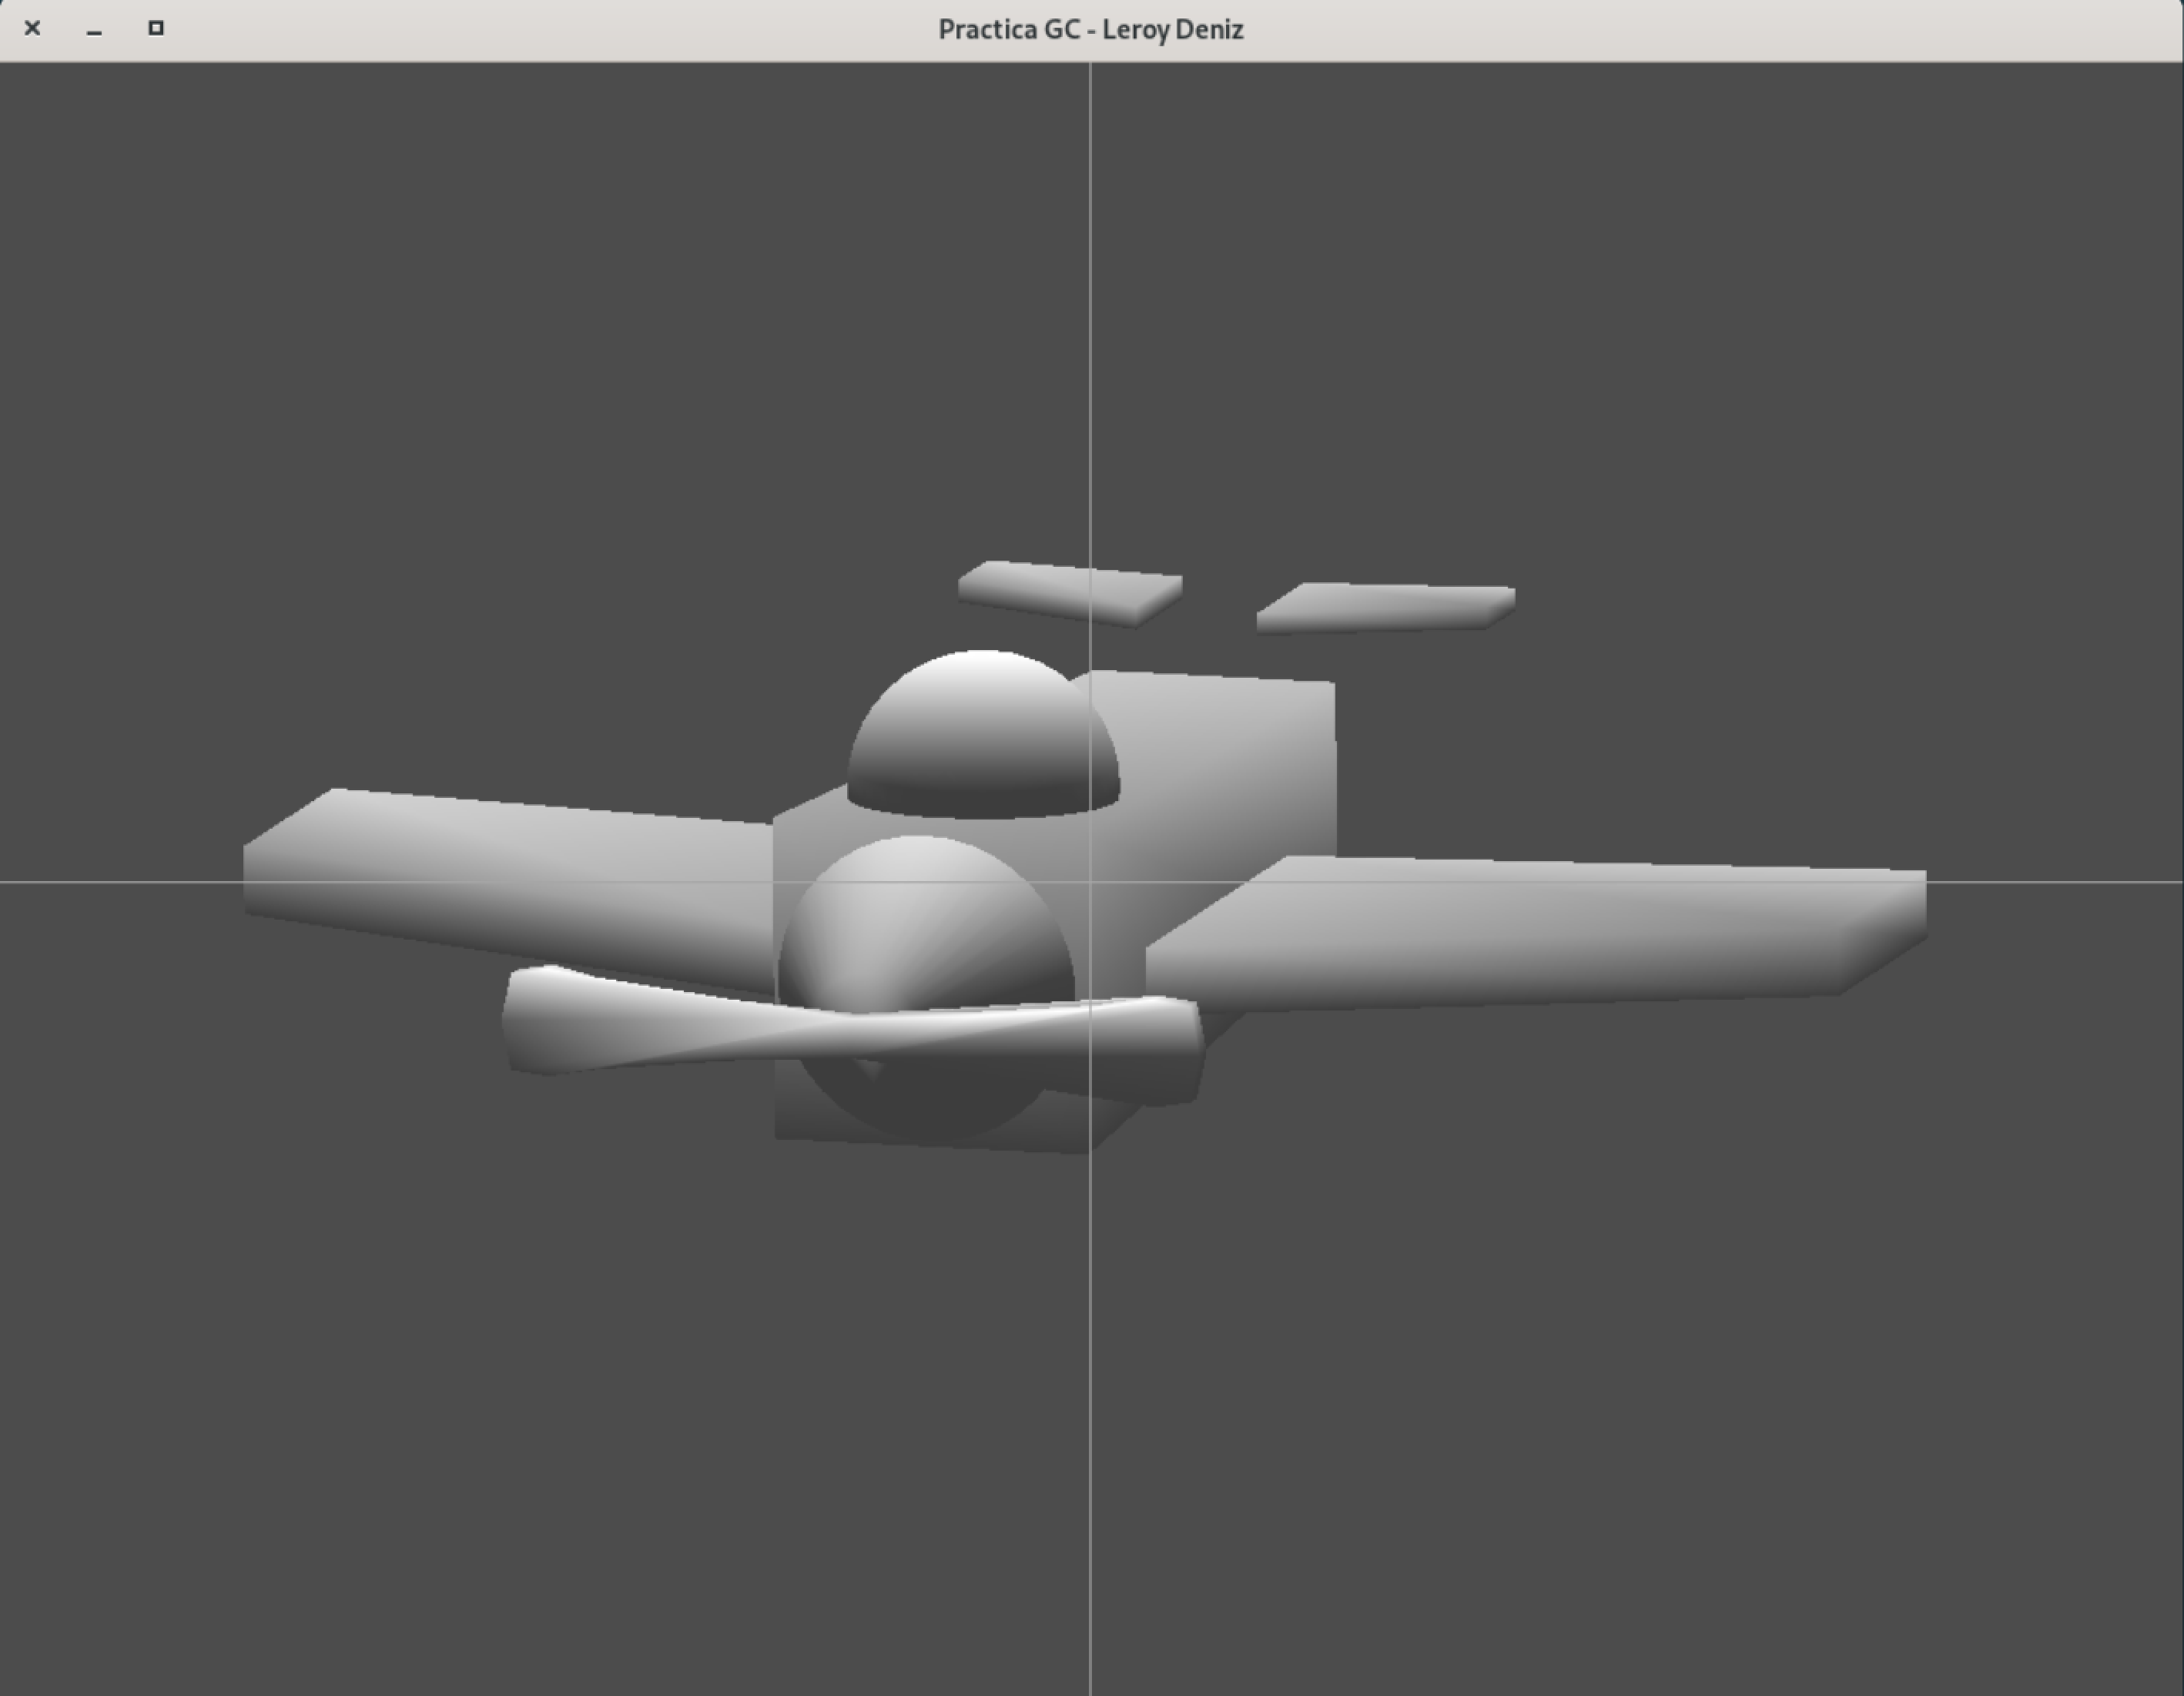
\includegraphics[width=.3\linewidth]{images/camara-simple}}\hfill
\subfloat[Objeto en perspectiva\label{fig:test2}]
  {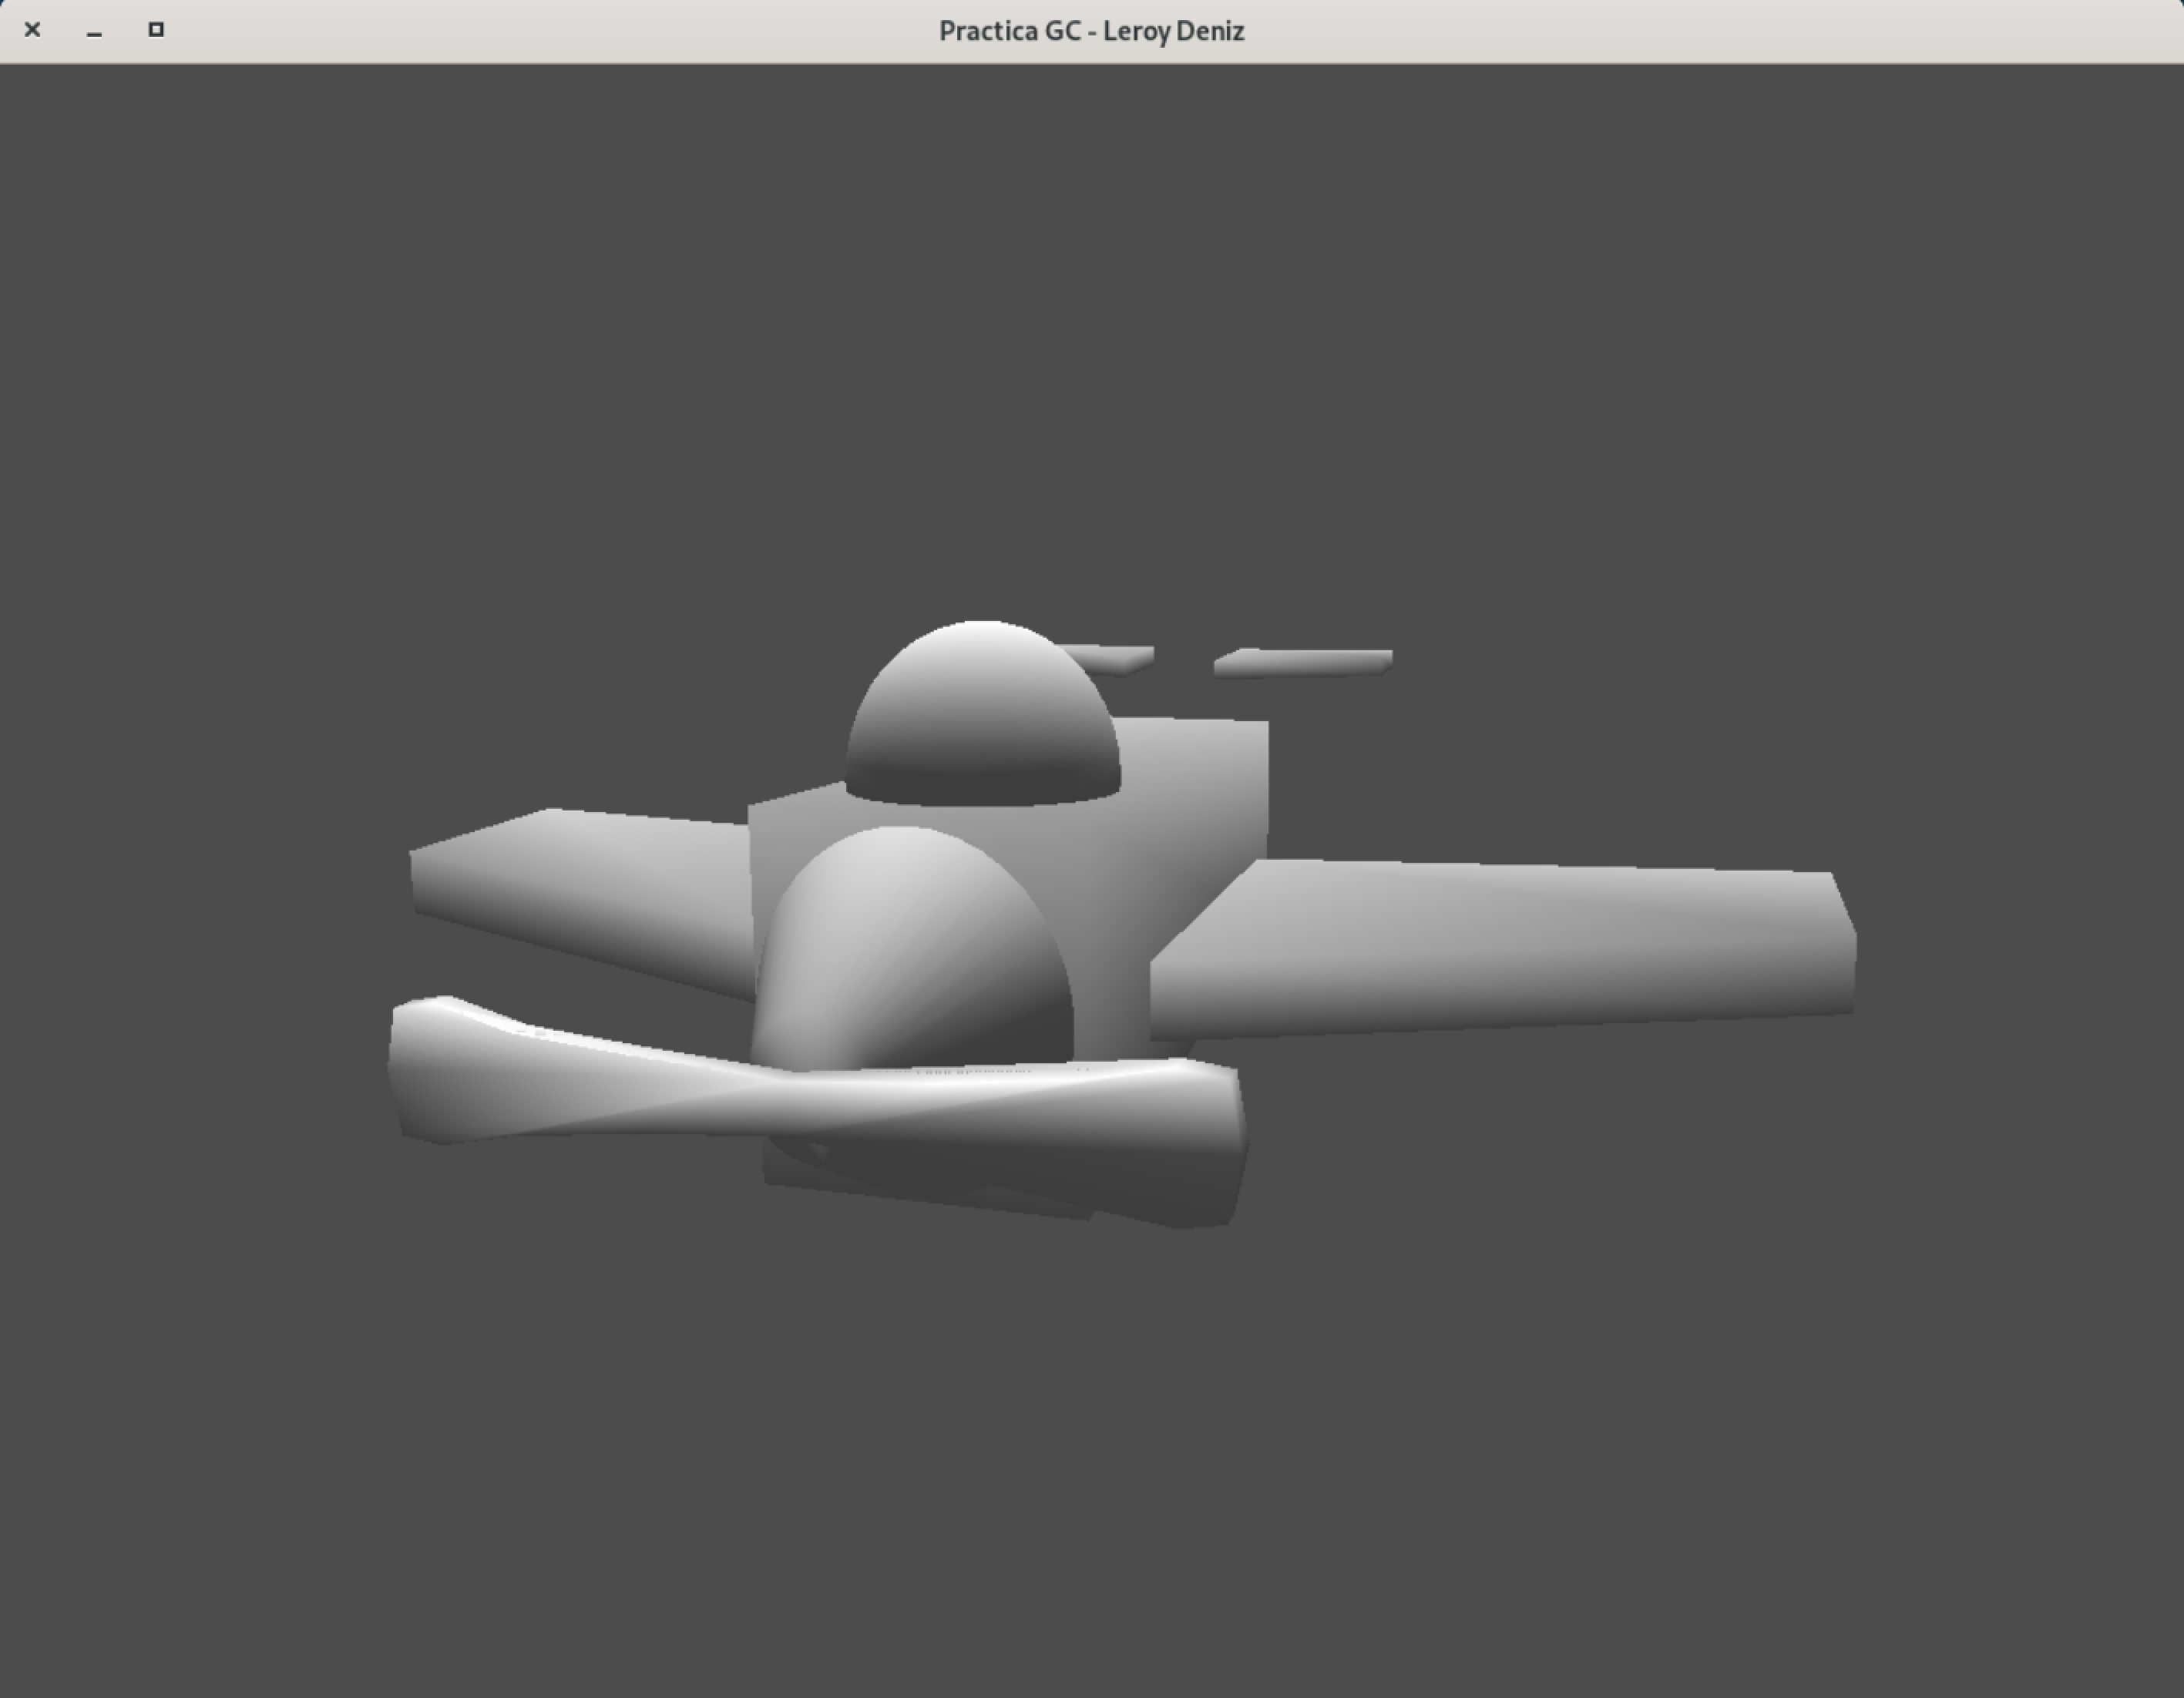
\includegraphics[width=.3\linewidth]{images/perspectiva}}\hfill
\subfloat[Perspectiva de ambos objetos\label{fig:test3}]
  {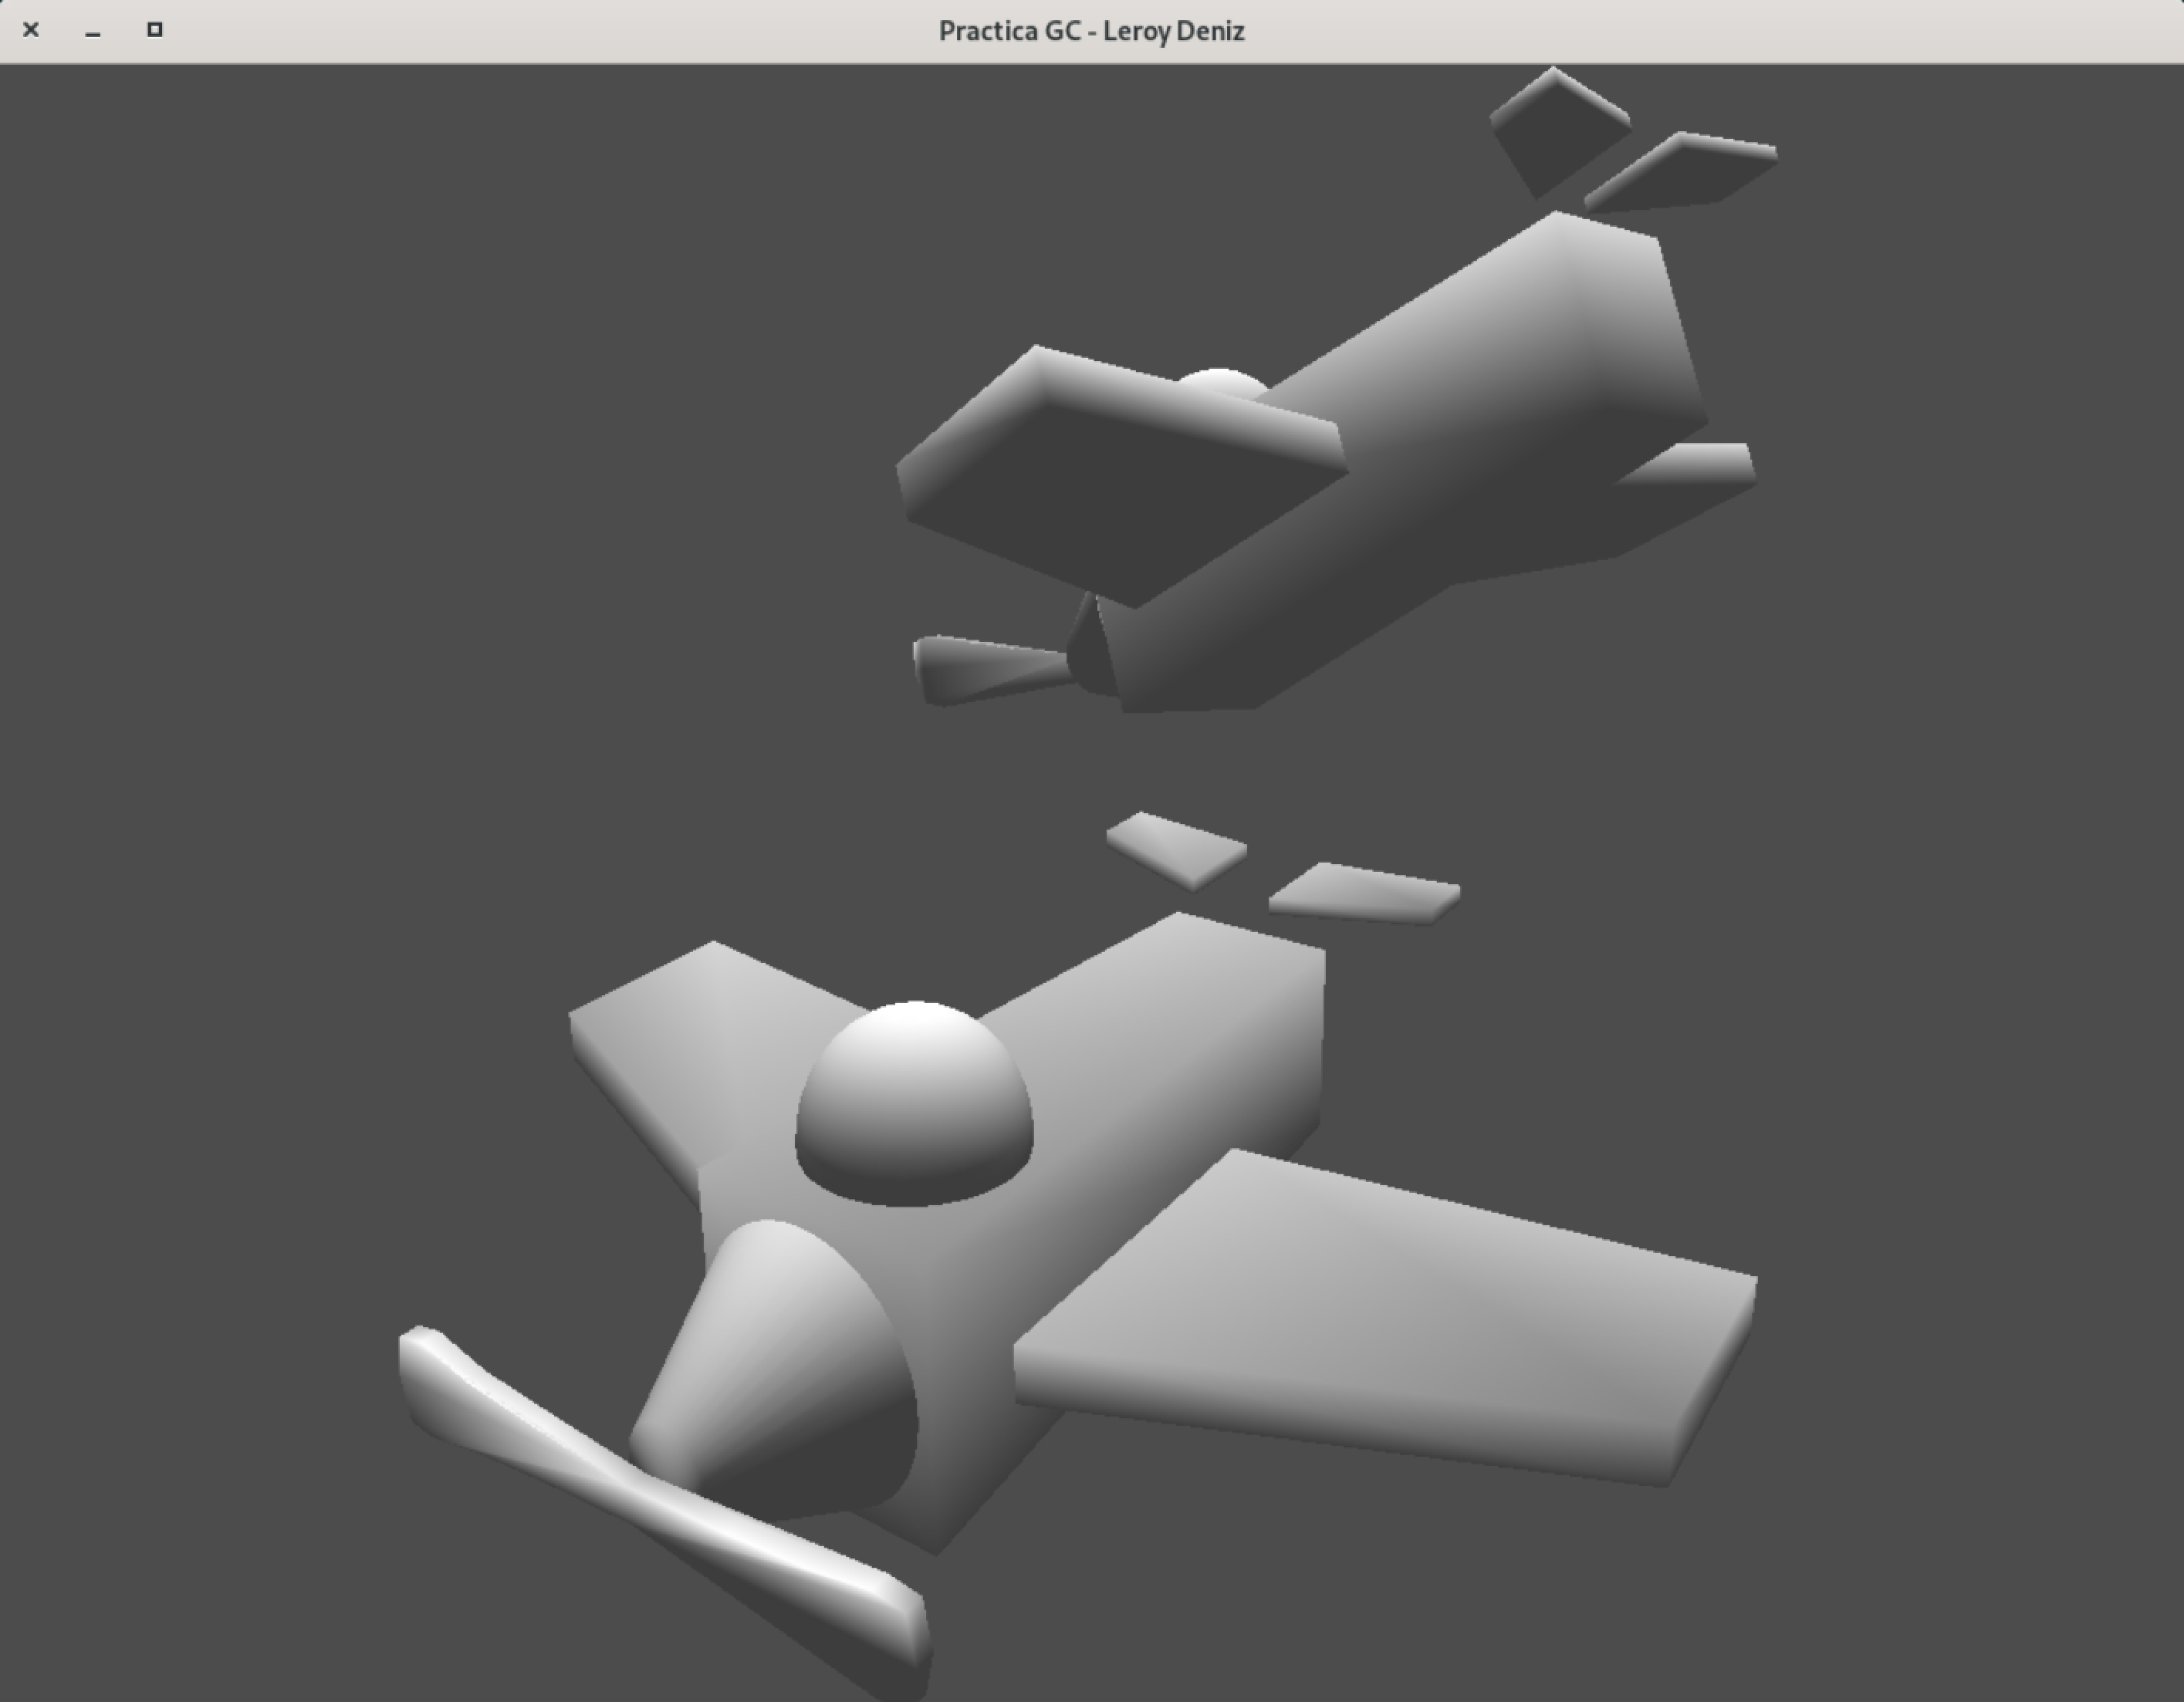
\includegraphics[width=.3\linewidth]{images/perspectiva-dos}}
\caption{Vistas de cámaras}
\end{figure}

\subsection{Tipos de cámara}

Tenemos definidos dos tipos de cámaras:

\begin{itemize}
\item \textbf{Cámara modo vuelo}: no mira un punto fijo y rota sobre su propio eje. Es capaz de mostrar todo el mundo 3D.
\item \textbf{Cámara modo análisis}: mira directamente al centro del objeto y rota sobre una esfera de radio fijo. Se centra en la inspección del propio objeto asociado.
\end{itemize}


\subsection{Inicialización de Cámara}

\begin{lstlisting}

/*********************************/
/*** INICIALIZACION CAMARA ***/
/*********************************/

camara *inicializarCamara(point3 e, point3 at, vector3 up) {
    camara *cam = (camara *) malloc(sizeof(camara));
    cam->e = e;
    cam->at = at;
    cam->up = up;
    calculaMatrizCamara(cam);
    return cam;
}

\end{lstlisting}

\newpage
\subsection{Rotación de Cámara}

\subsubsection{Decide el movimiento según la tecla}

\begin{lstlisting}

/*********************************/
/*** FUNCION DE ROTACION DE CAMARA ***/
/*********************************/

void rotacionCamara(int key, int x, int y) {
    GLdouble rota_respecto_x_plus[16] = {1, 0, 0, 0, 0, cos(0.05), sin(0.05), 0, 0, -sin(0.05),
    			 cos(0.05), 0, 0, 0, 0, 1};
    GLdouble rota_respecto_x_minus[16] = {1, 0, 0, 0, 0, cos(-0.05), sin(-0.05), 
    			0, 0, -sin(-0.05), cos(-0.05), 0, 0, 0, 0, 1};

    GLdouble rota_respecto_y_plus[16] = {cos(0.05), 0, -sin(0.05), 0, 0, 1, 0, 0, sin(0.05), 
    			0, cos(0.05), 0, 0, 0, 0, 1};
    GLdouble rota_respecto_y_minus[16] = {cos(-0.05), 0, -sin(-0.05), 0, 0, 1, 0, 0, sin(-0.05), 
    			0, cos(-0.05), 0, 0, 0, 0, 1};

    GLdouble rota_respecto_z_plus[16] = {cos(0.05), sin(0.05), 0, 0, -sin(0.05), cos(0.05), 
    			0, 0, 0, 0, 1, 0, 0, 0, 0, 1};
    GLdouble rota_respecto_z_minus[16] = {cos(-0.05), sin(-0.05), 0, 0, -sin(-0.05), cos(-0.05), 
    			0, 0, 0, 0, 1, 0, 0, 0, 0, 1};

    if (key == GLUT_KEY_UP) {
        multiplicaMatrizCamara(rota_respecto_x_plus);
    } else if (key == GLUT_KEY_LEFT) {
        multiplicaMatrizCamara(rota_respecto_y_minus);
    } else if (key == GLUT_KEY_DOWN) {
        multiplicaMatrizCamara(rota_respecto_x_minus);
    } else if (key == GLUT_KEY_RIGHT) {
        multiplicaMatrizCamara(rota_respecto_y_plus);
    } else if (key == GLUT_KEY_PAGE_UP) {
        multiplicaMatrizCamara(rota_respecto_z_minus);
    } else if (key == GLUT_KEY_PAGE_DOWN) {
        multiplicaMatrizCamara(rota_respecto_z_plus);
    }

}

/****************************************/
/*** ROTACION CAMARA VUELO ***/
/****************************************/

void ejecutaRotacionCamaraVuelo(int key) {
    if (key == GLUT_KEY_UP) {
        rotacionCamaraVuelo(_selected_camera, 1, 0, 0);
    } else if (key == GLUT_KEY_DOWN) {
        rotacionCamaraVuelo(_selected_camera, -1, 0, 0);
    } else if (key == GLUT_KEY_LEFT) {
        rotacionCamaraVuelo(_selected_camera, 0, -1, 0);
    } else if (key == GLUT_KEY_RIGHT) {
        rotacionCamaraVuelo(_selected_camera, 0, 1, 0);
    } else if (key == GLUT_KEY_PAGE_UP) {
        rotacionCamaraVuelo(_selected_camera, 0, 0, 1);
    } else if (key == GLUT_KEY_PAGE_DOWN) {
        rotacionCamaraVuelo(_selected_camera, 0, 0, -1);

    }
}

/*******************************************/
/*** ROTACION CAMARA ANALISIS ***/
/*******************************************/

void ejecutaRotacionCamaraAnalisis(int key) {
    if (key == GLUT_KEY_UP) {
        rotacionCamaraAnalisis(_selected_camera, 1, 0, 0);
    } else if (key == GLUT_KEY_DOWN) {
        rotacionCamaraAnalisis(_selected_camera, -1, 0, 0);
    } else if (key == GLUT_KEY_LEFT) {
        rotacionCamaraAnalisis(_selected_camera, 0, -1, 0);
    } else if (key == GLUT_KEY_RIGHT) {
        rotacionCamaraAnalisis(_selected_camera, 0, 1, 0);
    } else if (key == GLUT_KEY_PAGE_UP) {
        rotacionCamaraAnalisis(_selected_camera, 0, 0, 1);
    } else if (key == GLUT_KEY_PAGE_DOWN) {
        rotacionCamaraAnalisis(_selected_camera, 0, 0, -1);
    }
}

\end{lstlisting}

\subsubsection{Rotación de Cámara en Modo Vuelo}

\begin{lstlisting}
/*********************************/
/*** ROTACION DE CAMARA  VUELO ***/
/*********************************/
void rotacionCamaraVuelo(camara *camara, GLdouble x, GLdouble y, GLdouble z) {
    point3 newAt;

    vector3 x_cam = {camara->matrizCamara[0], camara->matrizCamara[4], camara->matrizCamara[8]};
    vector3 y_cam = {camara->matrizCamara[1], camara->matrizCamara[5], camara->matrizCamara[9]};
    vector3 z_cam = {camara->matrizCamara[2], camara->matrizCamara[6], camara->matrizCamara[10]};


    GLdouble matrizRotacion[16];
    glLoadIdentity();

    if (x != 0) {
        glRotated(2*x,x_cam.x,x_cam.y,x_cam.z);

    } else if (y != 0) {
        glRotated(2*y,y_cam.x,y_cam.y,y_cam.z);

    } else if (z != 0) {
        glRotated(2*z,z_cam.x,z_cam.y,z_cam.z);

    }
    glGetDoublev(GL_MODELVIEW_MATRIX, matrizRotacion);

    newAt.x = camara->at.x - camara->e.x;
    newAt.y = camara->at.y - camara->e.y;
    newAt.z = camara->at.z - camara->e.z;
    newAt=multiplicarMatrizPorPunto(matrizRotacion,newAt);

    newAt.x += camara->e.x;
    newAt.y += camara->e.y;
    newAt.z += camara->e.z;
    camara->at = newAt;
    camara->up=multiplicarMatrizPorVector(matrizRotacion,camara->up);
    calculaMatrizCamara(camara);
}


\end{lstlisting}

\subsubsection{Rotación de Cámara en Modo Análisis}

\begin{lstlisting}
/***********************************/
/*** ROTACION DE CAMARA ANALISIS ***/
/***********************************/
void rotacionCamaraAnalisis(camara *camara, GLdouble x, GLdouble y, GLdouble z) {
    point3 newPos;

    vector3 x_cam = {camara->matrizCamara[0], camara->matrizCamara[4], camara->matrizCamara[8]};
    vector3 y_cam = {camara->matrizCamara[1], camara->matrizCamara[5], camara->matrizCamara[9]};
    vector3 z_cam = {camara->matrizCamara[2], camara->matrizCamara[6], camara->matrizCamara[10]};


    GLdouble matrizRotacion[16];
    glLoadIdentity();

    if (x != 0) {
        glRotated(2*x,x_cam.x,x_cam.y,x_cam.z);
    } else if (y != 0) {
        glRotated(2*y,y_cam.x,y_cam.y,y_cam.z);
    } else if (z != 0) {
        glRotated(2*z,z_cam.x,z_cam.y,z_cam.z);
    }
    glGetDoublev(GL_MODELVIEW_MATRIX, matrizRotacion);

    newPos.x = camara->e.x - camara->at.x;
    newPos.y = camara->e.y - camara->at.y;
    newPos.z = camara->e.z - camara->at.z;
    newPos=multiplicarMatrizPorPunto(matrizRotacion,newPos);

    newPos.x += camara->at.x;
    newPos.y += camara->at.y;
    newPos.z += camara->at.z;
    camara->e = newPos;
    camara->up=multiplicarMatrizPorVector(matrizRotacion,camara->up);
    calculaMatrizCamara(camara);
}


\end{lstlisting}

\newpage
\subsection{Traslación de Cámara}

\subsubsection{Decide el movimiento según la tecla}

\begin{lstlisting}

/***********************************************/
/*** FUNCION DE TRASLACION CAMARA MODO VUELO ***/
/***********************************************/

void ejecutaTraslacionCamaraVuelo(int key) {
    if (key == GLUT_KEY_UP) {
        trasladarCamaraVuelo(_selected_camera, 0, 0.1, 0);
    } else if (key == GLUT_KEY_DOWN) {
        trasladarCamaraVuelo(_selected_camera, 0, -0.1, 0);
    } else if (key == GLUT_KEY_LEFT) {
        trasladarCamaraVuelo(_selected_camera, -0.1, 0, 0);
    } else if (key == GLUT_KEY_RIGHT) {
        trasladarCamaraVuelo(_selected_camera, 0.1, 0, 0);
    } else if (key == GLUT_KEY_PAGE_UP) {
        trasladarCamaraVuelo(_selected_camera, 0, 0, 0.1);
    } else if (key == GLUT_KEY_PAGE_DOWN) {
        trasladarCamaraVuelo(_selected_camera, 0, 0, -0.1);

    }
}

/**************************************************/
/*** FUNCION DE TRASLACION CAMARA MODO ANALISIS ***/
/**************************************************/

void ejecutaTraslacionCamaraAnalisis(int key) {
    if (key == GLUT_KEY_UP) {
        trasladarCamaraAnalisis(_selected_camera, 0, 0.1, 0);
    } else if (key == GLUT_KEY_DOWN) {
        trasladarCamaraAnalisis(_selected_camera, 0, -0.1, 0);
    } else if (key == GLUT_KEY_LEFT) {
        trasladarCamaraAnalisis(_selected_camera, -0.1, 0, 0);
    } else if (key == GLUT_KEY_RIGHT) {
        trasladarCamaraAnalisis(_selected_camera, 0.1, 0, 0);
    } else if (key == GLUT_KEY_PAGE_UP) {
        trasladarCamaraAnalisis(_selected_camera, 0, 0, 0.1);
    } else if (key == GLUT_KEY_PAGE_DOWN) {
        trasladarCamaraAnalisis(_selected_camera, 0, 0, -0.1);

    }
}

\end{lstlisting}

\subsubsection{Traslación de Cámara en Modo Vuelo}

\begin{lstlisting}

/**************************************************/
/*** FUNCION DE TRASLACION CAMARA MODO VUELO ***/
/**************************************************/

void trasladarCamaraVuelo(camara *camara, GLdouble x, GLdouble y, GLdouble z) {
    vector3 x_cam = {camara->matrizCamara[0], camara->matrizCamara[4], camara->matrizCamara[8]};
    vector3 y_cam = {camara->matrizCamara[1], camara->matrizCamara[5], camara->matrizCamara[9]};
    vector3 z_cam = {camara->matrizCamara[2], camara->matrizCamara[6], camara->matrizCamara[10]};

    camara->e.x += x * x_cam.x + y * y_cam.x + z * z_cam.x;
    camara->e.y += x * x_cam.y + y * y_cam.y + z * z_cam.y;
    camara->e.z += x * x_cam.z + y * y_cam.z + z * z_cam.z;

    camara->at.x += x * x_cam.x + y * y_cam.x + z * z_cam.x;
    camara->at.y += x * x_cam.y + y * y_cam.y + z * z_cam.y;
    camara->at.z += x * x_cam.z + y * y_cam.z + z * z_cam.z;
    calculaMatrizCamara(camara);
}
\end{lstlisting}

\newpage
\subsubsection{Traslación de Cámara en Modo Análisis}

\begin{lstlisting}
/**************************************************/
/*** FUNCION DE TRASLACION CAMARA MODO ANALISIS ***/
/**************************************************/

void trasladarCamaraAnalisis(camara *camara, GLdouble x, GLdouble y, GLdouble z) {
    vector3 x_cam = {camara->matrizCamara[0], camara->matrizCamara[4], camara->matrizCamara[8]};
    vector3 y_cam = {camara->matrizCamara[1], camara->matrizCamara[5], camara->matrizCamara[9]};
    vector3 z_cam = {camara->matrizCamara[2], camara->matrizCamara[6], camara->matrizCamara[10]};

    camara->e.x += x * x_cam.x + y * y_cam.x + z * z_cam.x;
    camara->e.y += x * x_cam.y + y * y_cam.y + z * z_cam.y;
    camara->e.z += x * x_cam.z + y * y_cam.z + z * z_cam.z;
    calculaMatrizCamara(camara);
}
\end{lstlisting}


\subsection{Funciones de Proyección}

Tenemos dos tipos de proyección:

\begin{itemize}
\item \textbf{Paralela}: permite una visión del objeto con sus medidas proporcionales y su posición en el espacio.
\item \textbf{Proyección}: cambia la visión del objeto, los puntos del mismo que estén más cerca de la cámara se agrandan y aquellos que están más lejos, se muestran más pequeños.
\end{itemize}

\begin{lstlisting}
/************************************************************/
/*** FUNCION DE MODIFICACION DE VOLUMEN SEGUN PERSPECTIVA ***/
/************************************************************/

void ejecutaModificacionVolumen(int key) {
    if (proyeccion == PARALELA) {
        if (key == GLUT_KEY_UP) {
            _ortho_y_max += 0.1;
        } else if (key == GLUT_KEY_DOWN) {
            _ortho_y_max -= 0.1;
        } else if (key == GLUT_KEY_LEFT) {
            _ortho_x_max -= 0.1;
        } else if (key == GLUT_KEY_RIGHT) {
            _ortho_x_max += 0.1;
        } else if (key == GLUT_KEY_PAGE_UP) {
            _ortho_z_max -= 0.1;
            _ortho_z_min -= 0.1;
        } else if (key == GLUT_KEY_PAGE_DOWN) {
            _ortho_z_max += 0.1;
            _ortho_z_min += 0.1;
        }
    } else if (proyeccion == PERSPECTIVA) {
        if (key == GLUT_KEY_UP) {
            _frust_y_max += 0.005;
        } else if (key == GLUT_KEY_DOWN) {
            _frust_y_max -= 0.005;
        } else if (key == GLUT_KEY_LEFT) {
            _frust_x_max -= 0.005;
        } else if (key == GLUT_KEY_RIGHT) {
            _frust_x_max += 0.005;
        } else if (key == GLUT_KEY_PAGE_UP) {
            _frust_z_max -= 0.005;
            _frust_z_min -= 0.005;
        } else if (key == GLUT_KEY_PAGE_DOWN) {
            _frust_z_max += 0.005;
            _frust_z_min += 0.005;
        }
    }
}
\end{lstlisting}

\newpage
\subsection{Funciones auxiliares}

\subsubsection{Calcular matriz de cámara que mira directo al objeto}

\begin{lstlisting}

/***************************************************/
/*** CALCULA MATRIZ DE CAMARA QUE MIRA AL OBJETO ***/
/***************************************************/

void mirarObjeto(camara *cam, object3d *obj) {
    cam->at.x = obj->pMptr->M[12];
    cam->at.y = obj->pMptr->M[13];
    cam->at.z = obj->pMptr->M[14];
    calculaMatrizCamara(cam);
}


\end{lstlisting}


\subsubsection{Calcular matriz correspondiente a una cámara}

\begin{lstlisting}
/********************************/
/*** CALCULA MATRIZ DE CAMARA ***/
/********************************/

void calculaMatrizCamara(camara *camara) {
    glLoadIdentity();
    gluLookAt(camara->e.x, camara->e.y, camara->e.z, camara->at.x, camara->at.y, camara->at.z, 
    			camara->up.x, camara->up.y, camara->up.z);
    glGetDoublev(GL_MODELVIEW_MATRIX, camara->matrizCamara);
}
\end{lstlisting}









\newpage

\section{Luces}

\subsection{Introducción}

El objetivo de esta tercer etapa de la práctica es implementar los conceptos sobre luces, de manera de poder implementar un sistema de iluminación sobre el estado actual de la aplicación. Para esto, se realizan los cálculos sobre los vectores normales de los planos, incorporación de materiales a los objetos 3D y generar distintas instancias de objetos de iluminación que permitan, además, poder transformarse.
La aplicación permite encender y apagar luces, por defecto viene inicializado solamente el sol (F1 en el teclado). Aquí se adjuntan tres vistas, en la primera, cargado con el material básico en el momento en el que se carga el objeto al iniciar el programa. Luego apagando el sol y finalmente con el sol encendido y con el foco de color 6 (F6).

\begin{figure}[H]
\subfloat[Vista normal con sol\label{fig:test1}]
  {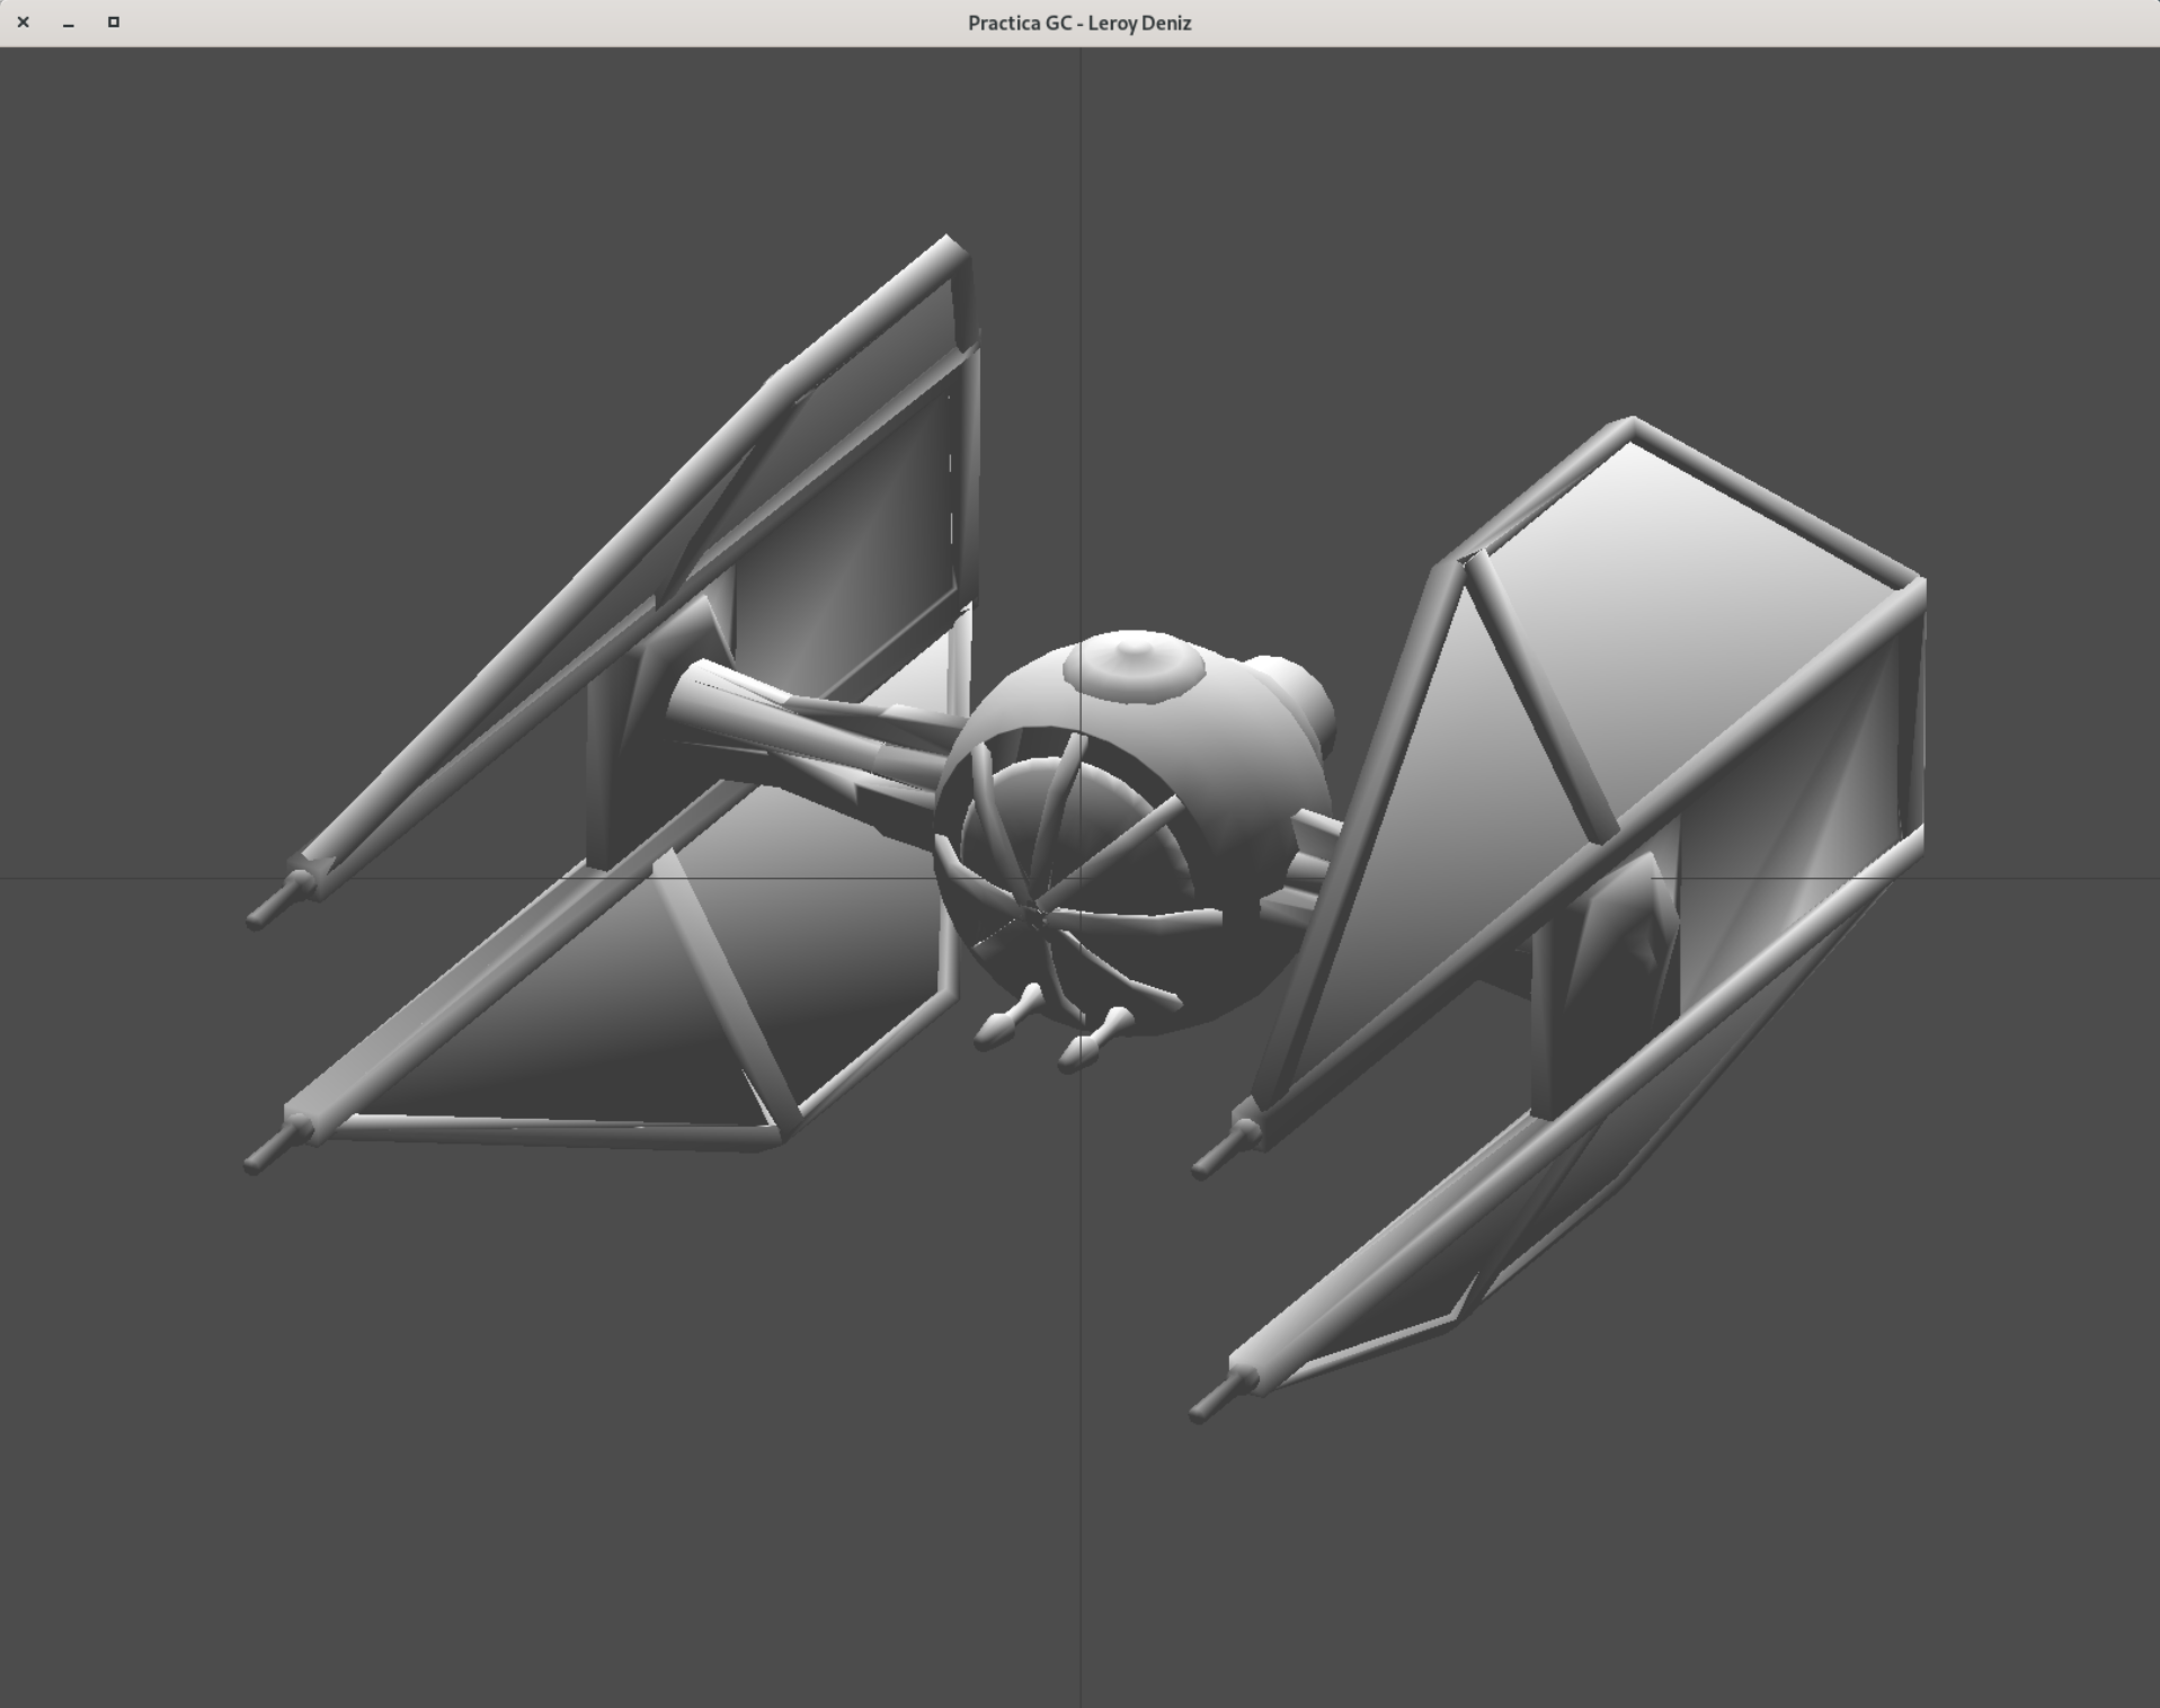
\includegraphics[width=.3\linewidth]{images/normal}}\hfill
\subfloat[Sin bombilla ni sol\label{fig:test2}]
  {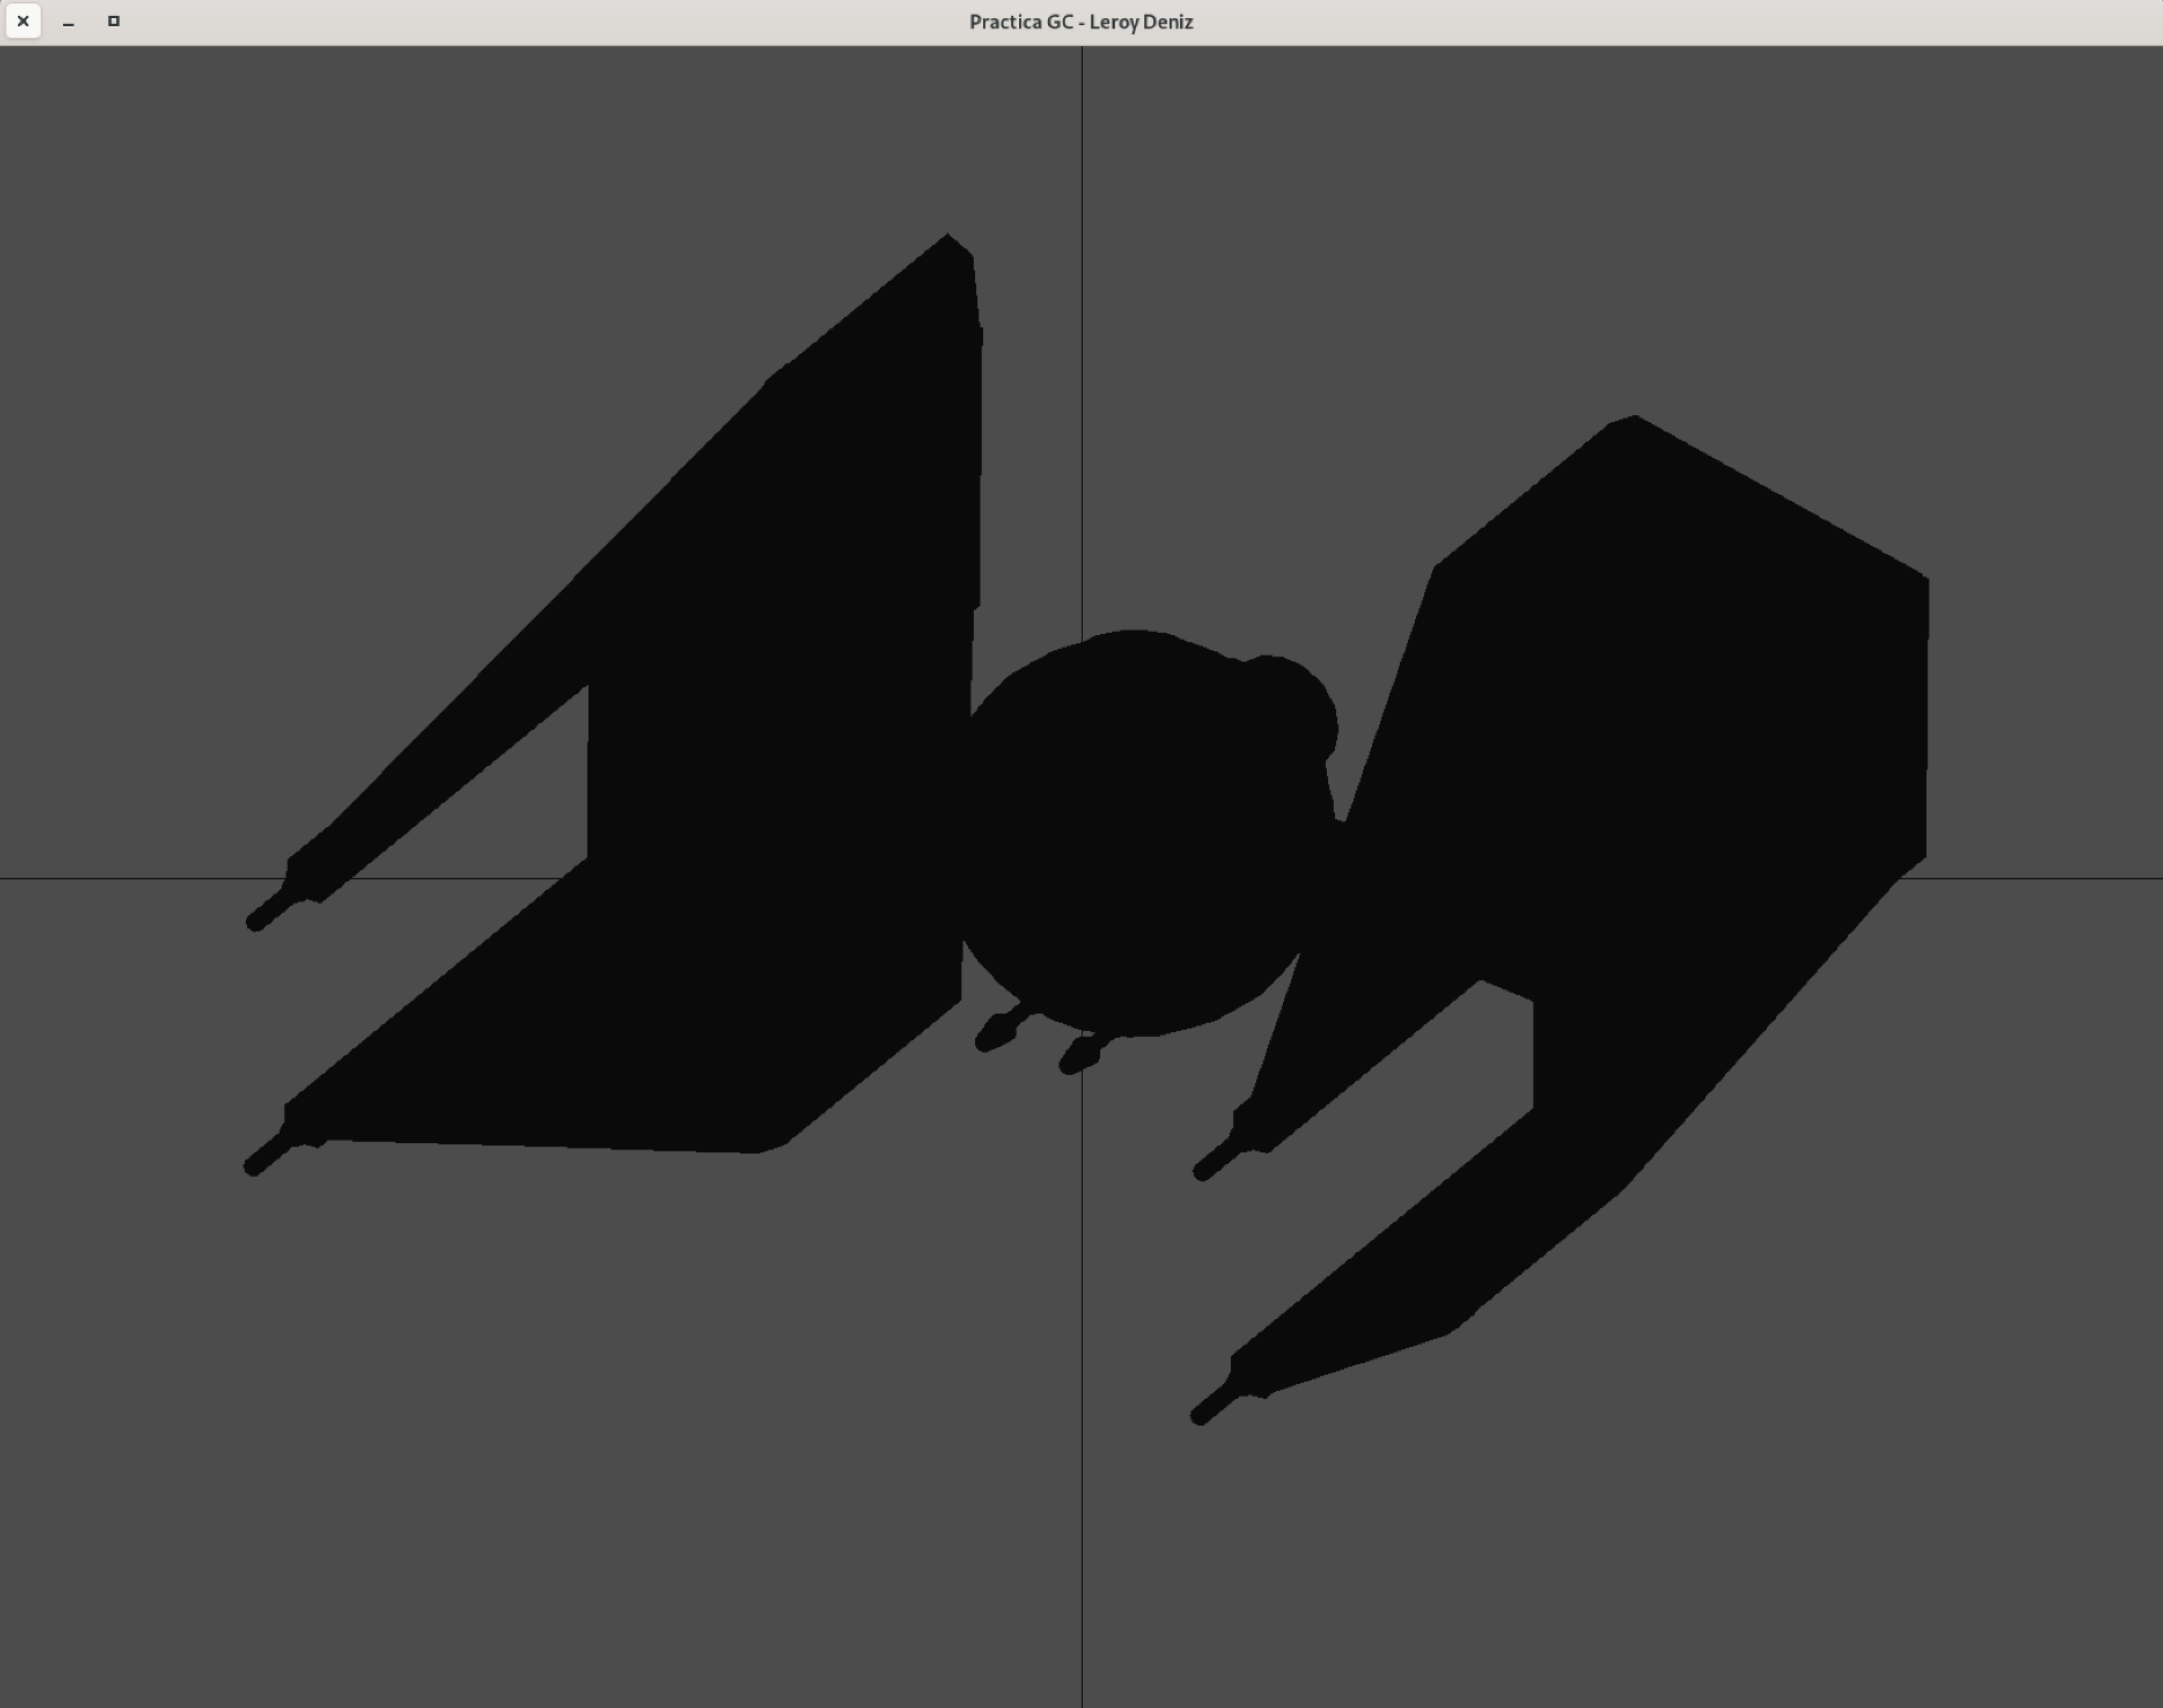
\includegraphics[width=.3\linewidth]{images/sinsol}}\hfill
\subfloat[Sol, bombilla y foco 6\label{fig:test3}]
  {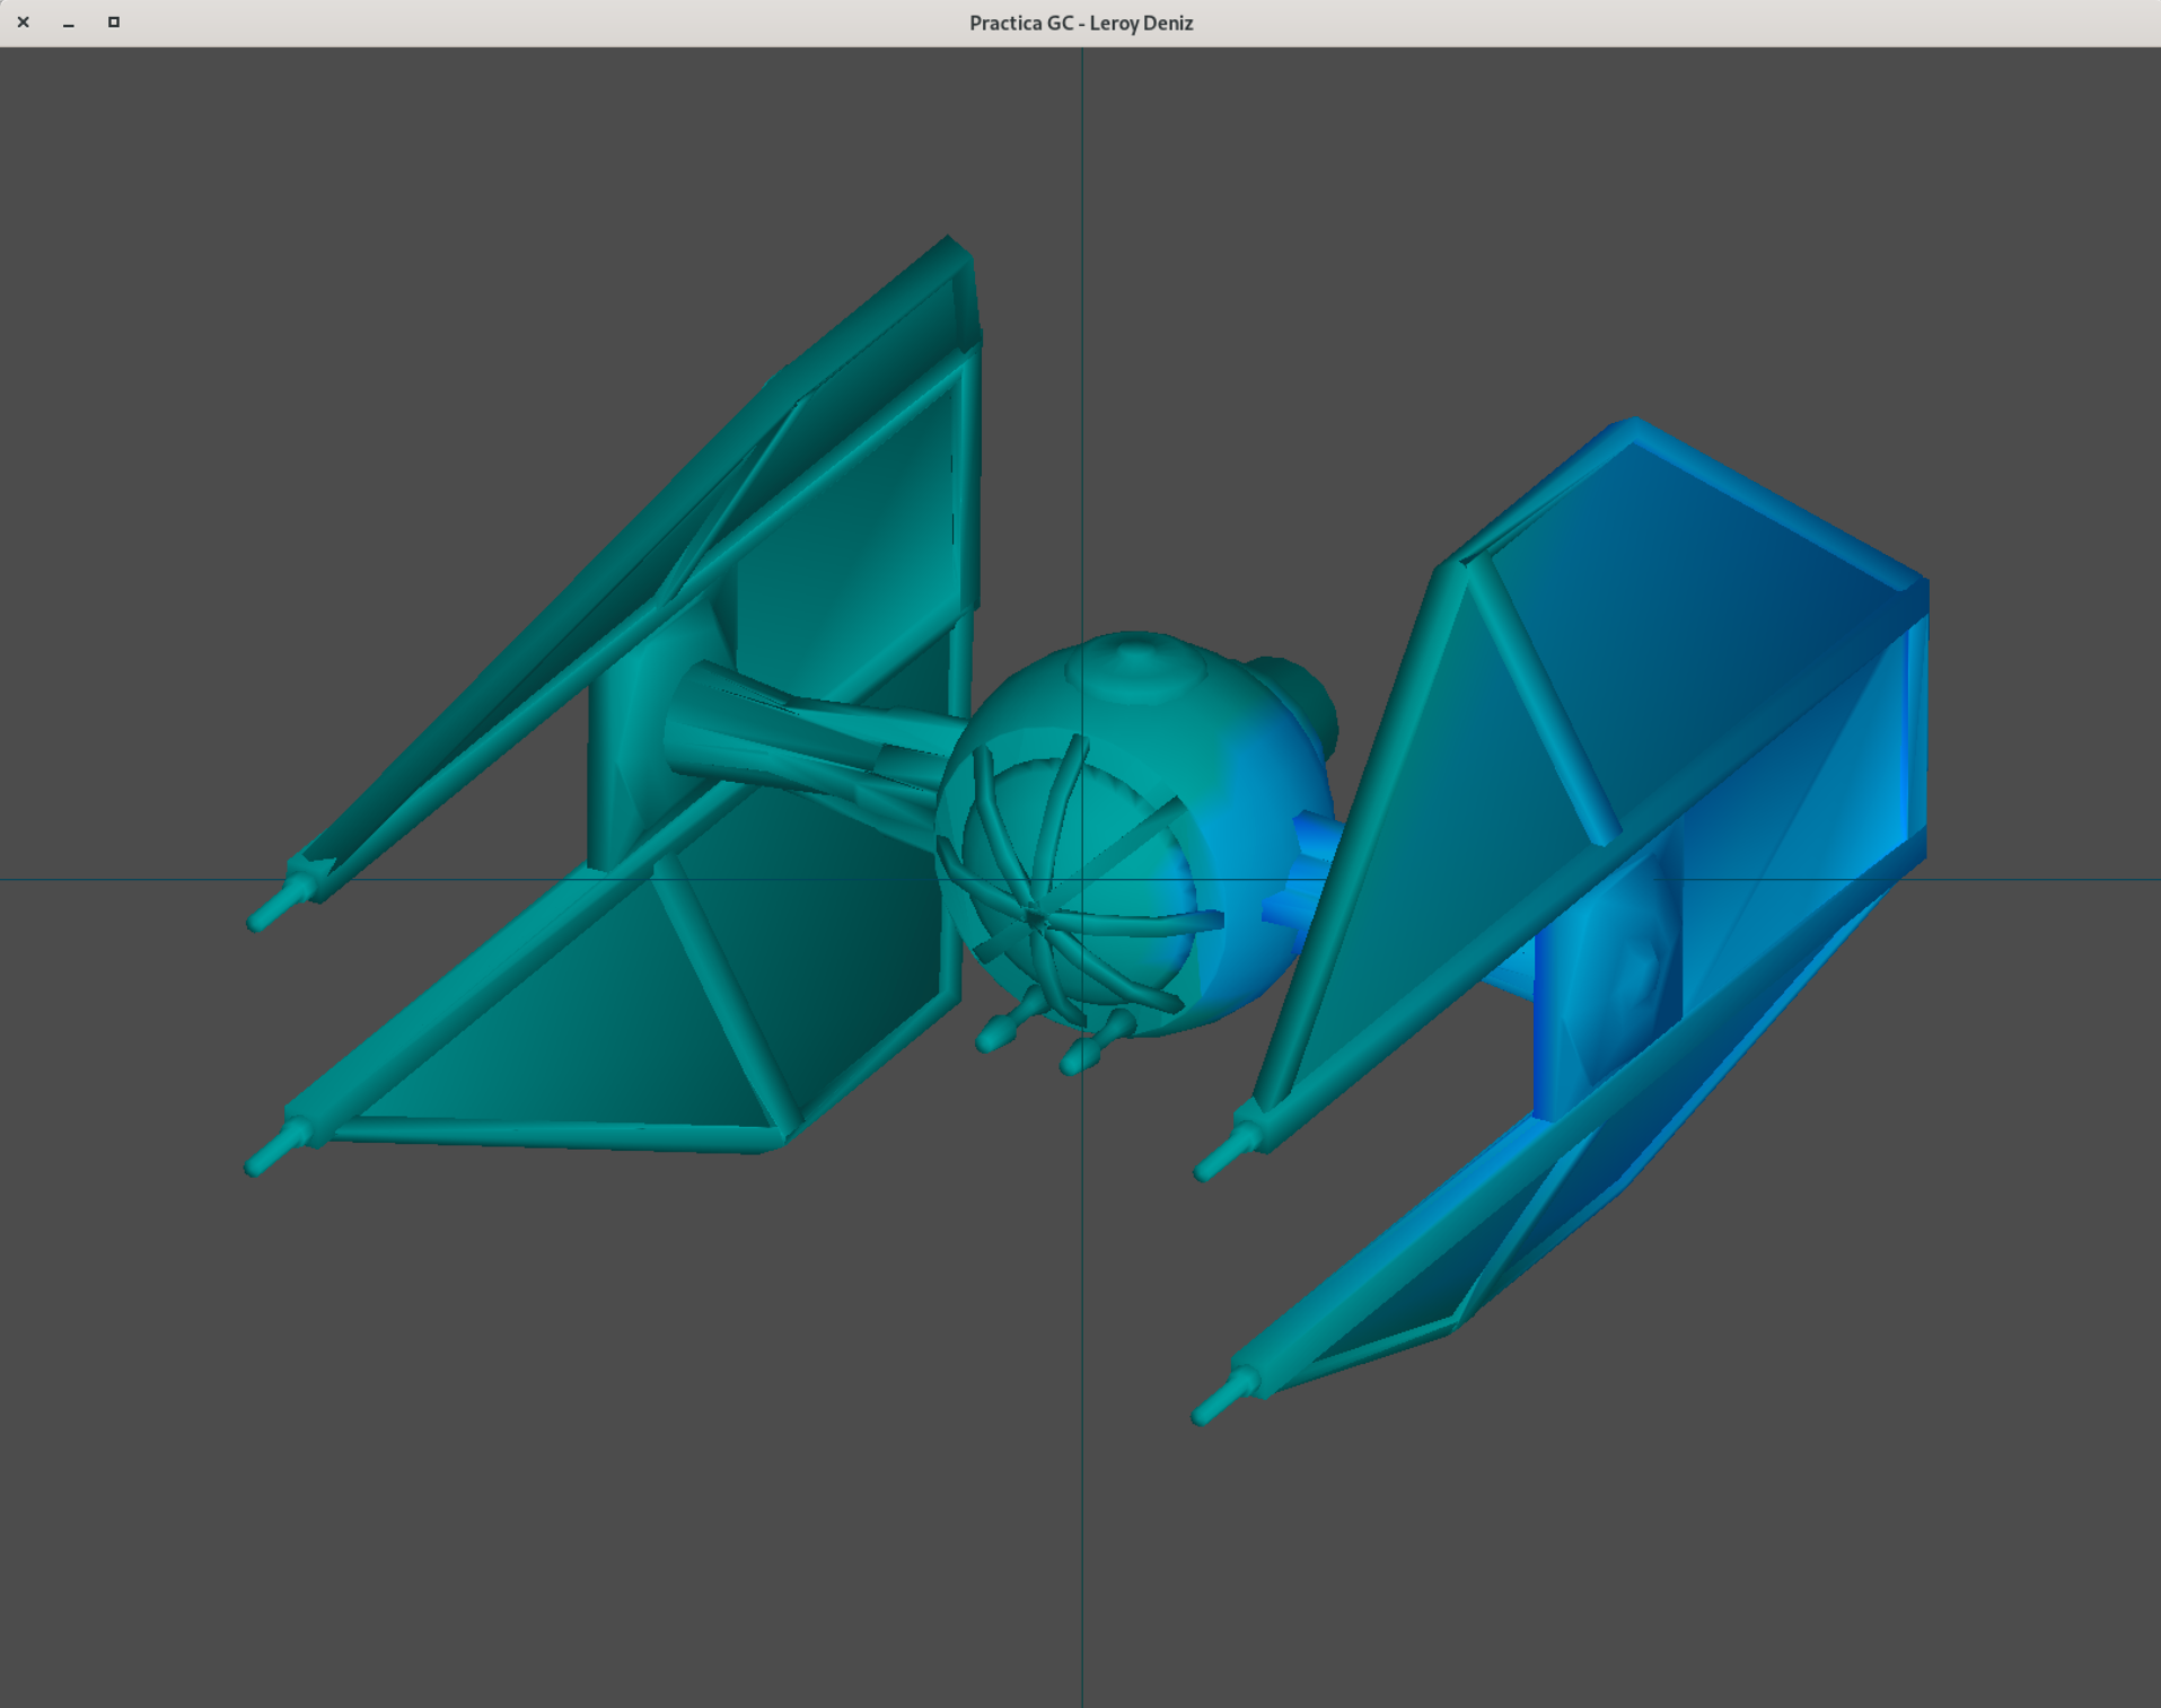
\includegraphics[width=.3\linewidth]{images/foco}}
\caption{Vistas del manejo de luces}
\end{figure}

\subsection{Tipos de luces}

Tenemos los siguientes tipos de objetos de luz:

\begin{itemize}
\item \textbf{Sol}: punto de luz fijo en el mundo, no se traslada ni se rota, siendo su dirección (0,1,0).
\item \textbf{Foco}: objeto de luz asociado al objeto, permite rotarlo y trasladarlo, siempre con el objeto 3D como su sistema de referencia al que está asociado. Cada objeto cargado tendrá su propio foco referenciándolo a este.
\item \textbf{Bombilla}: objeto de luz no asociado a ningún objeto en particular, permite rotarse y trasladarse libremente por el mundo, de forma global,  como no tiene sistema de referencia propio, utiliza el del mundo para moverse.
\end{itemize}

\subsection{Teclas para manejo de luces}

\begin{itemize}
\item \textbf{F1}: Prende y apaga el sol, por defecto está encendido.
\item \textbf{F2}: Prende y apaga el foco del objeto.
\item \textbf{F3}: Prende y apaga el objeto bombilla..
\end{itemize}

\subsection{Estructura del objeto luz}

Para la representación de la fuente de iluminación se definió una estructura $luz$, que representa cualquiera de los tipos mencionados anteriormente. 

\begin{lstlisting}
typedef struct luz{
    int tipo;
    int estado;
    GLfloat pos[4];
    GLfloat dir[3];
    GLfloat ambient[4];
    GLfloat diffuse[4];
    GLfloat specular[4];
    GLfloat ampFoco;
}luz;
\end{lstlisting}

Cada objeto de estos se compone por una serie de atributos que a continuación se definen.

\begin{itemize}
\item \textbf{tipo}: define si es un objeto de tipo sol, bombilla o foco; toma el valor del contenido de una de las tres constantes que representa al tipo de objeto de iluminación (SOL: 0, BOMBILLA: 1, FOCO: 2 ). 
\item \textbf{estado}: define si el objeto de iluminación estará encendido o no; toma el valor del contenido de una de las dos constantes que representa el estado (ENCENDIDA: 1, APAGADA: 0 ). 
\item \textbf{pos}: define la posición del objeto de iluminación en sus cuatro coordenadas. 
\item \textbf{dir}: define la dirección hacia donde mira el objeto de iluminación en sus cuatro coordenadas.
\item \textbf{ampFoco}: define la amplitud del foco hasta un ángulo llano.
\item \textbf{ambient}: luz ambiente.
\item \textbf{diffuse}: luz difusa.
\item \textbf{specular}: luz especular.
\end{itemize}

\subsection{Función de cambio entre bombilla a foco}

En caso que esté seleccionada la bombilla, tiene una dirección que no tiene el foco. Los atributos que componen el objeto luz no son utilizados en todos los tipos, sino que utilizan solamente aquellos que son parte del tipo específico.

\begin{lstlisting}

/********************************************/
/*** FUNCION DE CAMBIO DE BOMBILLA A FOCO ***/
/********************************************/

void cambiaFuenteLuz(int luzSeleccionada) {
    if (luzSeleccionada >= 3) {
        if (luces[luzSeleccionada].tipo==BOMBILLA){
            luces[luzSeleccionada].tipo=FOCO;
            luces[luzSeleccionada].ampFoco=45;
            luces[luzSeleccionada].dir[0]=0;
            luces[luzSeleccionada].dir[1]=-1;
            luces[luzSeleccionada].dir[2]=0;
        }
        else if(luces[luzSeleccionada].tipo==FOCO){
            luces[luzSeleccionada].tipo=BOMBILLA;
            luces[luzSeleccionada].ampFoco=180;
        }
    }
}
\end{lstlisting}

\subsection{Traslación de luz}

\subsubsection{Decide hacia dónde mover la luz}
\begin{lstlisting}

/************************************/
/*** FUNCION DE TRASLACION DE LUZ ***/
/************************************/

void ejecutaTraslacionLuz(int key) {
    if (key == GLUT_KEY_UP) {
        trasladarLuz(luzSeleccionada, 1, 0, 0);
    } else if (key == GLUT_KEY_DOWN) {
        trasladarLuz(luzSeleccionada, -1, 0, 0);
    } else if (key == GLUT_KEY_LEFT) {
        trasladarLuz(luzSeleccionada, 0, -1, 0);
    } else if (key == GLUT_KEY_RIGHT) {
        trasladarLuz(luzSeleccionada, 0, 1, 0);
    } else if (key == GLUT_KEY_PAGE_UP) {
        trasladarLuz(luzSeleccionada, 0, 0, 1);
    } else if (key == GLUT_KEY_PAGE_DOWN) {
        trasladarLuz(luzSeleccionada, 0, 0, -1);
    }
}

\end{lstlisting}


\subsubsection{Efectúa el movimiento}

\begin{lstlisting}

void trasladarLuz(int luzSeleccionada, GLfloat x, GLfloat y, GLfloat z) {
    point3 pos={x,y,z};
    point3 newPos;

    GLdouble matrizTraslacion[16];
    glLoadIdentity();
    glTranslatef(x, y, z);
    glGetDoublev(GL_MODELVIEW_MATRIX, matrizTraslacion);

    newPos=multiplicarMatrizPorPunto(matrizTraslacion,pos);
    luces[luzSeleccionada].pos[0]=newPos.x;
    luces[luzSeleccionada].pos[1]=newPos.y;
    luces[luzSeleccionada].pos[2]=newPos.z;
}

\end{lstlisting}

\newpage
\subsection{Rotación de luz}

\subsubsection{Decide hacia dónde rotar la luz}
\begin{lstlisting}

/**********************************/
/*** FUNCION DE ROTACION DE LUZ ***/
/**********************************/

void ejecutaRotacionLuz(int key) {
    if (key == GLUT_KEY_UP) {
        rotacionLuz(luzSeleccionada, 0, 10, 0);
    } else if (key == GLUT_KEY_DOWN) {
        rotacionLuz(luzSeleccionada, 0, -10, 0);
    } else if (key == GLUT_KEY_LEFT) {
        rotacionLuz(luzSeleccionada, -10, 0, 0);
    } else if (key == GLUT_KEY_RIGHT) {
        rotacionLuz(luzSeleccionada, 10, 0, 0);
    } else if (key == GLUT_KEY_PAGE_UP) {
        rotacionLuz(luzSeleccionada, 0, 0, 10);
    } else if (key == GLUT_KEY_PAGE_DOWN) {
        rotacionLuz(luzSeleccionada, 0, 0, -10);
    }
}

\end{lstlisting}

\subsubsection{Efectúa el movimiento}

\begin{lstlisting}

void rotacionLuz(int luzSeleccionada, GLfloat x, GLfloat y, GLfloat z) {
    point3 pos={x,y,z};
    point3 newPos;

    GLdouble matrizRotacion[16];
    glLoadIdentity();
    glRotatef(5.0, x, y, z);
    glGetDoublev(GL_MODELVIEW_MATRIX, matrizRotacion);

    newPos=multiplicarMatrizPorPunto(matrizRotacion,pos);
    luces[luzSeleccionada].pos[0]=newPos.x;
    luces[luzSeleccionada].pos[1]=newPos.y;
    luces[luzSeleccionada].pos[2]=newPos.z;
}

\end{lstlisting}





\newpage
\section{Materiales}
 
 La aplicación predefine el material $Jade$ por defecto, en este caso, no permite ir modificándolo, sino que podría ser una mejora a futuro. Para esto, se 

\subsection{Estructura}

Se predefine una estructura para el material en \texttt{definitions.h}.

\begin{lstlisting}
/****************************
 * Estructura de materiales *
 ****************************/
typedef struct material{
	GLfloat ambient[4];
	GLfloat diffuse[4];
	GLfloat specular[4];
	GLfloat shininess;
}material;
\end{lstlisting}

El objeto 3D tiene que contener también un puntero al material con el que está hecho.

\begin{lstlisting}
/****************************
 * Estructura de objetos    *
 ****************************/
struct object3d{
   ...
    material mt;			    /* definicion del material sobre el objeto */
    ...
};
\end{lstlisting}


\subsection{Inicialización}

El objeto tiene entonces definido un material, por lo que en el archivo \texttt{display.c} hay que inicializarlo antes de empezar a dibujar. Vamos a inicializar los colores de $Jade$ en la estructura $material$ asociada, que se utilizará para pintar el objeto.

\begin{lstlisting}
	aux_obj->mt.ambient[0] = 0.135;
	aux_obj->mt.ambient[1] = 0.2225;
	aux_obj->mt.ambient[2] = 0.1575;
	aux_obj->mt.ambient[3] = 1;

	aux_obj->mt.diffuse[0] = 0.54;
	aux_obj->mt.diffuse[1] = 0.89;
	aux_obj->mt.diffuse[2] = 0.63;
	aux_obj->mt.diffuse[3] = 1;

	aux_obj->mt.specular[0] = 0.316228;
	aux_obj->mt.specular[1] = 0.316228;
	aux_obj->mt.specular[2] = 0.316228;
	aux_obj->mt.specular[3] = 1;

	aux_obj->mt.shininess = 0.2;
\end{lstlisting}

Se le indica a $OpenGL$ los parámetros de esta textura.

\begin{lstlisting}
	glMaterialfv(GL_FRONT, GL_AMBIENT, aux_obj->mt.ambient);
	glMaterialfv(GL_FRONT, GL_DIFFUSE, aux_obj->mt.diffuse);
	glMaterialfv(GL_FRONT, GL_SPECULAR, aux_obj->mt.specular);
	glMaterialf(GL_FRONT, GL_SHININESS, aux_obj->mt.shininess);
\end{lstlisting}

A este punto, el objeto será dibujado con la textura predefinida, aunque sin poder cambiarse.

\newpage

\section{Función de control de teclado}

\subsection{Manejo de opciones de teclado}

\begin{lstlisting}
void keyboard(unsigned char key, int x, int y) {

    char *fname = malloc(sizeof(char) * 128);
    int read = 0;
    object3d *auxiliar_object = 0;
    GLdouble wd, he, midx, midy;

    switch (key) {
    
        case 'k':
        case 'K':
            printf("\n*** ACTIVADO : MODO CAMARA ***\n");
            modo = CAMARA;
            break;
            
        case 'o':
        case 'O':
            printf("\n*** ACTIVADO : MODO OBJETOS ***\n");
            modo = OBJETO;
            break;
            
        case 'b':
        case 'B':
            printf("\n*** ACTIVADO : MODO ROTACION ***\n");
            estado = ROTACION;
            break;
            
        case 't':
        case 'T':
            if (modo == OBJETO) {
                printf("\n*** ACTIVADO : MODO ESCALADO ***\n");
                estado = ESCALADO;
            } else if (modo == CAMARA) {
                printf("\n*** ACTIVADO : MODO VOLUMEN ***\n");
                estado = VOLUMEN;
            }
            break;
            
        case 'p':
        case 'P':
            if (proyeccion == PARALELA) {
                printf("\n*** ACTIVADO : PROYECCION PERSPECTIVA ***\n");
                proyeccion = PERSPECTIVA;
            } else if (proyeccion == PERSPECTIVA) {
                printf("\n*** ACTIVADO : PROYECCION PARALELA ***\n");
                proyeccion = PARALELA;
            }
            break;
            
        case 'm':
        case 'M':
            printf("\n*** ACTIVADO : MODO TRASLACION ***\n");
            estado = TRASLACION;
            break;
            
        case 'g':
        case 'G':
            if (modo == OBJETO) {
                printf("\n*** ACTIVADO : REFERENCIA GLOBAL ***\n");
                referencia = GLOBAL;
            } else if (modo == CAMARA) {
                printf("\n*** ACTIVADO : MODO ANALISIS ***\n");
                modoCamara = ANALISIS;
                mirarObjeto(_selected_camera, _selected_object);
            }
            break;
            
        case 'l':
        case 'L':
            if (modo == OBJETO) {
                printf("\n*** ACTIVADO : REFERENCIA LOCAL ***\n");
                referencia = LOCAL;
            } else if (modo == CAMARA) {
                printf("\n*** ACTIVADO : MODO VUELO ***\n");
                modoCamara = VUELO;
            }
            break;
            
        case '.':
            if (modo == OBJETO) {
                print_matrix(_selected_object->pMptr->M);
            } else
                print_matrix(_selected_camera->matrizCamara);
            break;
            
        case 48:
            printf("\n*** ACTIVADO : CAMBIAR FUENTE DE LUZ ***\n");
            cambiaFuenteLuz(luzSeleccionada);
            break;
            
        case 49: /* <1> */
            printf("\n*** ACTIVADA : LUZ 0 ***\n");
            luzSeleccionada = 0;
            break;
            
        case 50: /* <2> */
            printf("\n*** ACTIVADA : LUZ 1 ***\n");
            luzSeleccionada = 1;
            break;
            
        case 51: /* <3> */
            printf("\n*** ACTIVADA : LUZ 2 ***\n");
            luzSeleccionada = 2;
            break;
            
        case 52: /* <4> */
            printf("\n*** ACTIVADA : LUZ 3 ***\n");
            luzSeleccionada = 3;
            break;
            
        case 53: /* <5> */
            printf("\n*** ACTIVADA : LUZ 4 ***\n");
            luzSeleccionada = 4;
            break;
            
        case 54: /* <6> */
            printf("\n*** ACTIVADA : LUZ 5 ***\n");
            luzSeleccionada = 5;
            break;
            
        case 55: /* <7> */
            printf("\n*** ACTIVADA : LUZ 6 ***\n");
            luzSeleccionada = 6;
            break;
            
        case 56: /* <8> */
            printf("\n*** ACTIVADA : LUZ 7 ***\n");
            luzSeleccionada = 7;
            break;
            
        case 'a':
        case 'A':
            modo = LUZ;
            printf("\n*** ACTIVADO : MODO LUZ ***\n");
            break;
            
        case 'f':
        case 'F':
            /*Ask for file*/
            printf("%s", KG_MSSG_SELECT_FILE);
            scanf("%s", fname);
            /*Allocate memory for the structure and read the file*/
            auxiliar_object = (object3d *) malloc(sizeof(object3d));
            read = read_wavefront(fname, auxiliar_object);
            switch (read) {
                /*Errors in the reading*/
                case 1:
                    printf("%s: %s\n", fname, KG_MSSG_FILENOTFOUND);
                    break;
                case 2:
                    printf("%s: %s\n", fname, KG_MSSG_INVALIDFILE);
                    break;
                case 3:
                    printf("%s: %s\n", fname, KG_MSSG_EMPTYFILE);
                    break;
                case 0:
                    /*Insert the new object in the list*/
                    auxiliar_object->siguiente = _first_object;
                    _first_object = auxiliar_object;
                    _selected_object = _first_object;
                    auxiliar_object->pMptr = (elem_Matriz *) malloc(sizeof(elem_Matriz));
                    auxiliar_object->containerNodePtr = (elem_Matriz *) malloc(sizeof(elem_Matriz));
                    printf("%s\n", KG_MSSG_FILEREAD);
                    glMatrixMode(GL_MODELVIEW);
                    glLoadIdentity();
                    glGetDoublev(GL_MODELVIEW_MATRIX, auxiliar_object->pMptr->M);
                    auxiliar_object->pMptr->siguiente = 0;
                    break;
            }
            break;
            
        case 'c':
        case 'C':
            inversa(_selected_object->pMptr->M, _selected_camera->matrizCamara);
            printf("\n*** ACTIVADA : CAMARA DE OBJETO ***\n");
            break;
            
        case 9: /* <TAB> */
            if (_selected_object != 0) {
                if (_selected_object->siguiente != 0)
                    _selected_object = _selected_object->siguiente;
                else
                    _selected_object = _first_object;
                /*The selection is circular, thus if we move out of the list we go back to the first element*/
            } else _selected_object = _first_object;
            break;
            
        case 127: /* <SUPR> */
            	/*Erasing an object depends on whether it is the first one or not*/
		if(_first_object != 0 ) {
		    if (_selected_object == _first_object) {
		        /*To remove the first object we just set the first as the current's siguiente*/
		        _first_object = _first_object->siguiente;
		        /*Once updated the pointer to the first object it is save to free the memory*/
		        free(_selected_object);
		        /*Finally, set the selected to the new first one*/
		        _selected_object = _first_object;
		    } else {
		        /*In this case we need to get the previous element to the one we want to erase*/
		        auxiliar_object = _first_object;
		        while (auxiliar_object->siguiente != _selected_object)
		            auxiliar_object = auxiliar_object->siguiente;
		        /*Now we bypass the element to erase*/
		        auxiliar_object->siguiente = _selected_object->siguiente;
		        /*free the memory*/
		        free(_selected_object);
		        /*and update the selection*/
		        _selected_object = auxiliar_object;
		    }
		}
		break;

        case '-':
            if (glutGetModifiers() == GLUT_ACTIVE_CTRL) {
                /*Increase the projection plane; compute the new dimensions*/
                wd = (_ortho_x_max - _ortho_x_min) / KG_STEP_ZOOM;
                he = (_ortho_y_max - _ortho_y_min) / KG_STEP_ZOOM;
                /*In order to avoid moving the center of the plane, we get its coordinates*/
                midx = (_ortho_x_max + _ortho_x_min) / 2;
                midy = (_ortho_y_max + _ortho_y_min) / 2;
                /*The the new limits are set, keeping the center of the plane*/
                _ortho_x_max = midx + wd / 2;
                _ortho_x_min = midx - wd / 2;
                _ortho_y_max = midy + he / 2;
                _ortho_y_min = midy - he / 2;
            } else if (modo == OBJETO && estado == ESCALADO) {
                escaladoHomogeneo(1);
            } else if (luces[luzSeleccionada].tipo==FOCO) {
                if(luces[luzSeleccionada].ampFoco<=0){
                    printf("\n*** AVISO : MODIFICACION NO PERMITIDA, AMPLITUD = 0 ***\n");
                }else
                    printf("DISMINUYENDO ANGULO DE APERTURA %f\n", luces[luzSeleccionada].ampFoco--);
            }
            break;

        case '+':
            if (glutGetModifiers() == GLUT_ACTIVE_CTRL) {
                /*Increase the projection plane; compute the new dimensions*/
                wd = (_ortho_x_max - _ortho_x_min) * KG_STEP_ZOOM;
                he = (_ortho_y_max - _ortho_y_min) * KG_STEP_ZOOM;
                /*In order to avoid moving the center of the plane, we get its coordinates*/
                midx = (_ortho_x_max + _ortho_x_min) * 2;
                midy = (_ortho_y_max + _ortho_y_min) * 2;
                /*The the new limits are set, keeping the center of the plane*/
                _ortho_x_max = midx + wd / 2;
                _ortho_x_min = midx - wd / 2;
                _ortho_y_max = midy + he / 2;
                _ortho_y_min = midy - he / 2;
            } else if (modo == OBJETO && estado == ESCALADO) {
                escaladoHomogeneo(0);

            } else if (luces[luzSeleccionada].tipo==FOCO) {
                if(luces[luzSeleccionada].ampFoco>=90){
                    printf("\n*** AVISO : MODIFICACION NO PERMITIDA, AMPLITUD = 90 ***\n");
                }else
                    printf("AUMENTANDO ANGULO DE APERTURA %f\n", luces[luzSeleccionada].ampFoco++);
            }
            break;
        case 26: /* <CTRL + Z>- undo */
            if (glutGetModifiers() == GLUT_ACTIVE_CTRL) {
                if (_selected_object) {
                    if (_selected_object->pMptr->siguiente != 0) {
                        redo();
                    } else
                        printf("\n*** AVISO : NADA MAS PARA DESHACER ***\n");
                }
            }
            break;
            
        case 24:/* <CTRL + X> - redo*/
            if (glutGetModifiers() == GLUT_ACTIVE_CTRL) {
                if (_selected_object->containerNodePtr->siguiente != 0) {
                    auxPtr = _selected_object->containerNodePtr->siguiente;
                    _selected_object->containerNodePtr->siguiente = _selected_object->pMptr;
                    _selected_object->pMptr = _selected_object->containerNodePtr;
                    _selected_object->containerNodePtr = auxPtr;
                } else {
                    printf("\n*** AVISO : NADA MAS PARA REHACER ***\n");
                }
            }
            break;

        case '?':
            print_help();
            break;

        case 27: /* <ESC> */
            exit(0);
            break;
            
        default:
            /*In the default case we just print the code of the key. This is usefull to define new cases*/
            printf("%d %c\n", key, key);
    }
    /*In case we have do any modification affecting the displaying of the object, we redraw them*/
    glutPostRedisplay();
}

\end{lstlisting}

\newpage
\subsection{Manejo de teclas Fn y flechas}

\begin{lstlisting}
/*****************************************/
/*** FUNCION DE ACCION DE FLECHAS Y FX ***/
/*****************************************/

void k_arrow(int key, int x, int y) {
    switch (key) {
    
        case GLUT_KEY_F9:
            if (luces_activadas == 1) {
                printf("\n*** ACTIVADO : LUCES ***\n");
                glEnable(GL_LIGHTING);
                luces_activadas = 0;
            } else {
                printf("\n*** DESACTIVADO : LUCES ***\n");
                glDisable(GL_LIGHTING);
                luces_activadas = 1;
            }
            break;
            
        case GLUT_KEY_F1:
            if (luces[0].estado==APAGADA) {
                printf("\n*** ACTIVADA : LUZ  - SOL ***\n");
                glEnable(GL_LIGHT0);
                luces[0].estado=ENCENDIDA;
            } else {
                printf("\n*** DESACTIVADA : LUZ  - SOL ***\n");
                glDisable(GL_LIGHT0);
                luces[0].estado=APAGADA;
            }
            break;
            
        case GLUT_KEY_F2:
            if (luces[1].estado==APAGADA) {
                printf("\n*** ACTIVADA : LUZ 1 - BOMBILLA ***\n");
                glEnable(GL_LIGHT1);
                luces[1].estado=ENCENDIDA;
            } else {
                printf("\n*** DESACTIVADA : LUZ 1 - BOMBILLA ***\n");
                glDisable(GL_LIGHT1);
                luces[1].estado=APAGADA;
            }
            break;
            
        case GLUT_KEY_F3:
            if (luces[2].estado==APAGADA) {
                printf("\n*** ACTIVADA : LUZ 2 - FOCO OBJETO ***\n");
                glEnable(GL_LIGHT2);
                luces[2].estado=ENCENDIDA;
            } else {
                printf("\n*** DESACTIVADA : LUZ 2 - FOCO OBJETO ***\n");
                glDisable(GL_LIGHT2);
                luces[2].estado=APAGADA;
            }
            break;
            
        case GLUT_KEY_F4:
            if (luces[3].estado==APAGADA) {
                printf("\n*** ACTIVADA : LUZ 3 ***\n");
                glEnable(GL_LIGHT3);
                luces[3].estado=ENCENDIDA;
            } else {
                printf("\n*** DESACTIVADA : LUZ 3 ***\n");
                glDisable(GL_LIGHT3);
                luces[3].estado=APAGADA;
            }
            break;
            
        case GLUT_KEY_F5:
            if (luces[4].estado==APAGADA) {
                printf("\n*** ACTIVADA : LUZ 4 ***\n");
                glEnable(GL_LIGHT4);
                luces[4].estado=ENCENDIDA;
            } else {
                printf("\n*** DESACTIVADA : LUZ 4 ***\n");
                glDisable(GL_LIGHT4);
                luces[4].estado=APAGADA;
            }
            break;
            
        case GLUT_KEY_F6:
            if (luces[5].estado==APAGADA) {
                printf("\n*** ACTIVADA : LUZ 5 ***\n");
                glEnable(GL_LIGHT5);
                luces[5].estado=ENCENDIDA;
            } else {
                printf("\n*** DESACTIVADA : LUZ 5 ***\n");
                glDisable(GL_LIGHT5);
                luces[5].estado=APAGADA;
            }
            break;
            
        case GLUT_KEY_F7:
            if (luces[6].estado==APAGADA) {
                printf("\n*** ACTIVADA : LUZ 6 ***\n");
                glEnable(GL_LIGHT6);
                luces[6].estado=ENCENDIDA;
            } else {
                printf("\n*** DESACTIVADA : LUZ 6 ***\n");
                glDisable(GL_LIGHT6);
                luces[6].estado=APAGADA;
            }
            break;
            
        case GLUT_KEY_F8:
            if (luces[7].estado==APAGADA) {
                printf("\n*** ACTIVADA : LUZ 7 ***\n");
                glEnable(GL_LIGHT7);
                luces[7].estado=ENCENDIDA;
            } else {
                printf("\n*** DESACTIVADA : LUZ 7 ***\n");
                glDisable(GL_LIGHT7);
                luces[7].estado=APAGADA;
            }
            break;
            
        case GLUT_KEY_F12:
            if (shading == SMOOTH) {
                shading = FLAT;
                glShadeModel(GL_FLAT);
            } else {
                shading = SMOOTH;
                glShadeModel(GL_SMOOTH);
            }
            break;
    }
    
    if (modo == OBJETO) {
	if(_selected_object!=0) {
		if (referencia == LOCAL) {
		    if (estado == ROTACION)
		        ejecutaRotacion(key, x, y);
		    else if (estado == ESCALADO)
		        ejecutaEscalado(key, x, y);
		    else if (estado == TRASLACION)
		        ejecutaTraslacion(key, x, y);
		} else {
		    if (estado == ROTACION)
		        ejecutaRotacionGlobal(key, x, y);
		    else if (estado == ESCALADO)
		        ejecutaEscaladoGlobal(key, x, y);
		    else if (estado == TRASLACION)
		        ejecutaTraslacionGlobal(key, x, y);
		    }
		}
	 } else if (modo == CAMARA) {
		if (estado == ROTACION) {
		    printf("\n*** CAMARA : ROTANDO CAMARA ***\n");
		    if (modoCamara == VUELO)
		        ejecutaRotacionCamaraVuelo(key);
		    else if (modoCamara == ANALISIS) {
		        ejecutaRotacionCamaraAnalisis(key);
		    }
		} else if (estado == TRASLACION) {
		    printf("\n*** TRASLACION : MOVIENDO CAMARA ***\n");
		    if (modoCamara == VUELO)
		        ejecutaTraslacionCamaraVuelo(key);
		    else if (modoCamara == ANALISIS)
		        ejecutaTraslacionCamaraAnalisis(key);
		} else if (estado == VOLUMEN) {
		    printf("\n*** VOLUMEN : MODIFICANDO VOLUMEN ***\n");
		    ejecutaModificacionVolumen(key);
		}
	    } else if (modo == LUZ) {
		if (luzSeleccionada != SOL) {
		    if (estado == TRASLACION) {
		        ejecutaTraslacionLuz(key);
		    }
		    else if(estado==ROTACION){
		        ejecutaRotacionLuz(key);
		    }
		}
	
    }
    glutPostRedisplay();
}

\end{lstlisting}







\newpage

\section{Funciones auxiliares transversales}

Aquí se detalla el código de las funciones auxiliares de la aplicación, que permiten el manejo de las órdenes desde la función principal.

\subsection{Calcular producto vectorial}

\begin{lstlisting}
vector3 productoVectorial(vector3 u, vector3 v) {
    vector3 res;
    res.x = u.y * v.z - v.y * u.z;
    res.y = v.x * u.z - u.x * v.z;
    res.z = u.x * v.y - v.x * u.y;
    return res;
}

\end{lstlisting}

\subsection{Calcular matriz inversa}

Como son matrices ortonormales, su matriz inversa es igual a su matriz traspuesta: $A^{-1} = A^T$

\begin{lstlisting}

/******************************************************/
/*** FUNCION PARA CALCULAR MATRIZ INVERSA) ***/
/******************************************************/

void inversa(GLdouble m[16], GLdouble *inv) {
    // Gldouble inv[16];
    inv[0] = m[0];
    inv[1] = m[4];
    inv[2] = m[8];
    inv[3] = (GLdouble) 0;
    inv[4] = m[1];
    inv[5] = m[5];
    inv[6] = m[9];
    inv[7] = (GLdouble) 0;
    inv[8] = m[2];
    inv[9] = m[6];
    inv[10] = m[10];
    inv[11] = (GLdouble) 0;
    inv[12] = -m[12];
    inv[13] = -m[13];
    inv[14] = -m[14];
    inv[15] = (GLdouble) 1;
}

\end{lstlisting}

\subsection{Multiplicar matriz (modifica el sistema de referencia local)}

Para modificar el sistema de referencia local, el producto de la última matriz de transformación asociada al objeto y la nueva matriz de transformación, debe ser multiplicando la por la derecha.

\begin{lstlisting}

/******************************************************/
/*** FUNCION DE MODIFICACION LOCAL (POR LA DERECHA) ***/
/******************************************************/

void multiplicaMatriz(GLdouble matriz[]) {
    mPtr = (elem_Matriz *) malloc(sizeof(elem_Matriz));
    glLoadMatrixd(_selected_object->pMptr->M);
    glMultMatrixd(matriz);
    glGetDoublev(GL_MODELVIEW_MATRIX, mPtr->M);
    mPtr->siguiente = _selected_object->pMptr;
    _selected_object->pMptr = mPtr;
}

\end{lstlisting}

\subsection{Multiplicar matriz (modifica el sistema de referencia global)}

Para realizar una transformación en el sistema de referencia global,  se utiliza la función $glMultMatrix$, pero como se tiene que multiplicar por la izquierda, es necesario multiplicar primero a la matriz identidad por la matriz de transformación correspondiente al movimiento que se quiere realizar, para luego multiplicar ese contenido por la matriz del último movimiento realizado por el objeto y que se mantiene guardado en la lista del tipo $elem\_Matriz$.


\begin{lstlisting}

/*********************************************************/
/*** FUNCION DE MODIFICACION GLOBAL (POR LA IZQUIERDA) ***/
/*********************************************************/

void multiplicaMatrizGlobal(GLdouble matriz[]) {
    mPtr = (elem_Matriz *) malloc(sizeof(elem_Matriz));
    glLoadIdentity();
    glMultMatrixd(matriz);
    glMultMatrixd(_selected_object->pMptr->M);
    glGetDoublev(GL_MODELVIEW_MATRIX, mPtr->M);
    mPtr->siguiente = _selected_object->pMptr;
    _selected_object->pMptr = mPtr;
}

\end{lstlisting}

\subsection{Multiplicar matriz por punto}

\begin{lstlisting}
/***********************************/
/*** MULTIPLICA MATRIZ POR PUNTO ***/
/***********************************/

point3 multiplicarMatrizPorPunto(GLdouble m[16], point3 p) {
    point3 r;
    r.x = m[0] * p.x + m[4] * p.y + m[8] * p.z + m[12];
    r.y = m[1] * p.x + m[5] * p.y + m[9] * p.z + m[13];
    r.z = m[2] * p.x + m[6] * p.y + m[10] * p.z + m[14];
    return r;
}

\end{lstlisting}


\subsection{Multiplicar matriz por vector}

\begin{lstlisting}

/************************************/
/*** MULTIPLICA MATRIZ POR VECTOR ***/
/************************************/

vector3 multiplicarMatrizPorVector(GLdouble m[16], vector3 p) {
    vector3 r;
    r.x = m[0] * p.x + m[4] * p.y + m[8] * p.z;
    r.y = m[1] * p.x + m[5] * p.y + m[9] * p.z;
    r.z = m[2] * p.x + m[6] * p.y + m[10] * p.z;
    return r;
}

\end{lstlisting}










\newpage
\section{Conclusiones}

Aunque la aplicación está terminada, tiene ciertos aspectos que pueden ser mejorables en términos de optimización de código. Una mejora posible es ampliar la gama de materiales posibles en su implementación y no permitir la superposición de objetos.

Además, y quizá lo más importante, de cara a futuro habría que mejorar la documentación dentro del código para permitir seguir el flujo de trabajo de cara a posibles mejoras, ya que actualmente está restringido al conocimiento de quien desarrolla y no a una posible re utilización de código para proyectos futuros.


\begin{center}
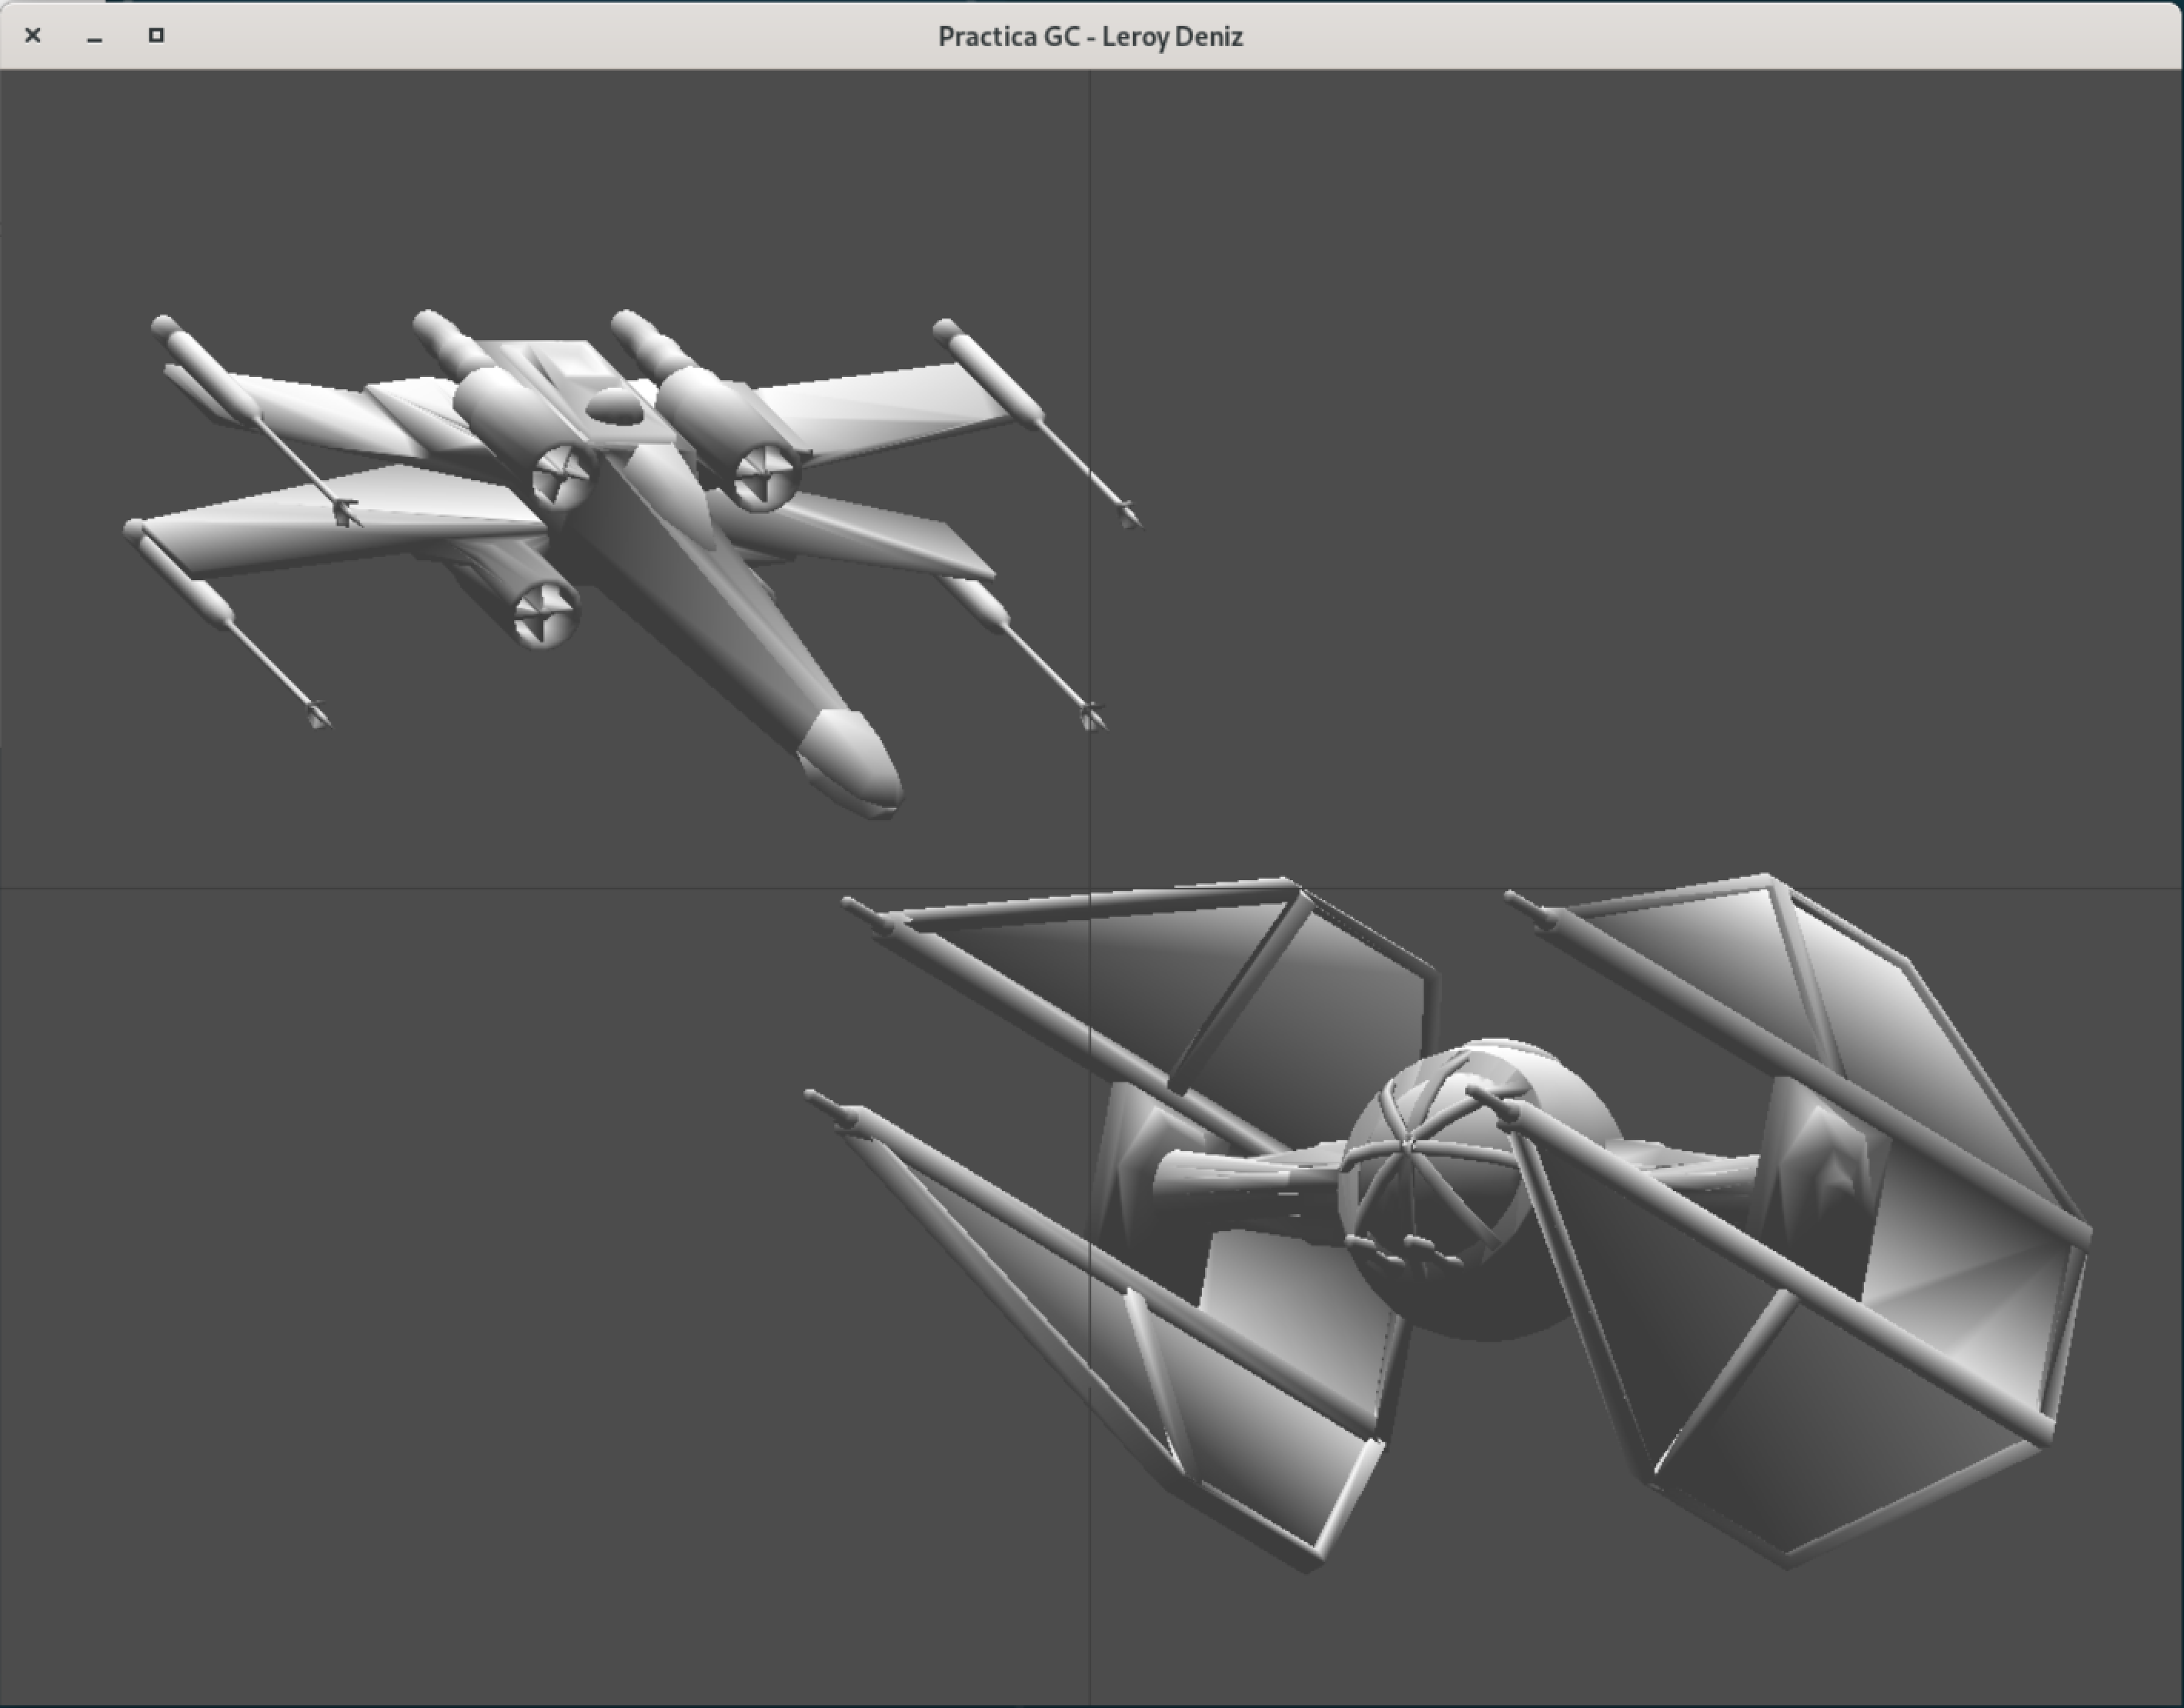
\includegraphics[width=14cm]{images/naves}
\end{center}





\newpage
\section{Bibliografía}

\begin{itemize}
\item Harris, J. W., \& Stöcker, H. (1998). \textit{Handbook of Mathematics and Computational Science (1998 ed.). } Springer.

\item Hearn, D., Baker, M., \& Carithers, W. (2010).  \textit{Computer Graphics with OpenGL (4th ed.).} Pearson.

\item Hughes, J., Dam, V. A., McGuire, M., Sklar, D., Foley, J., Feiner, S., \& Akeley, K. (2013). \textit{Computer Graphics: Principles and Practice (3rd Revised ed.).} Addison-Wesley Professional.

\item Preparata, F. P., \& Shamos, M. I. (2012). \textit{Computational Geometry.} Springer Publishing.

\item Shreiner, D., Sellers, G., Kessenich, J. M., Licea-Kane, B., \& Khronos \textit{OpenGL ARB Working Group. (2013).  OpenGL Programming Guide. } Addison-Wesley.
\end{itemize}

\end{document}
